\chapter{Ground segment}
Ground station design should complement the space segment, with large antenna gains and output power to allow the budget link to close. As the system is full-duplex, both uplink and downlink channels are separate and the design should allow to simultaneously operate transmit and receive. Block diagram of the designed ground station is shown in the figure \ref{gs_block_diagram}.
Due to the low sensitivity of the satellite receiver (\SI{-98}{\dBm}) uplink EIRP has to be very large, this is achieved by using high-power amplifier and antennas with high directional gain. For downlink, ground station has to compensate low transmit power of the satellite, by using high gain antennas and very sensitive receiver.

Ground station consists of not only the hardware but also software. Many parts of the system use Digital Signal Processing and Software-Defined Radio for data modulation/de-modulation, packet transmission etc. For the DSP tasks, GNUradio \cite{gnuradio} was selected and the tool for sampling-based signal processing.

Ground station is located on the building of Faculty of Electronics and Information Technology, Warsaw University of Technology.



\begin{figure}
    \centering
    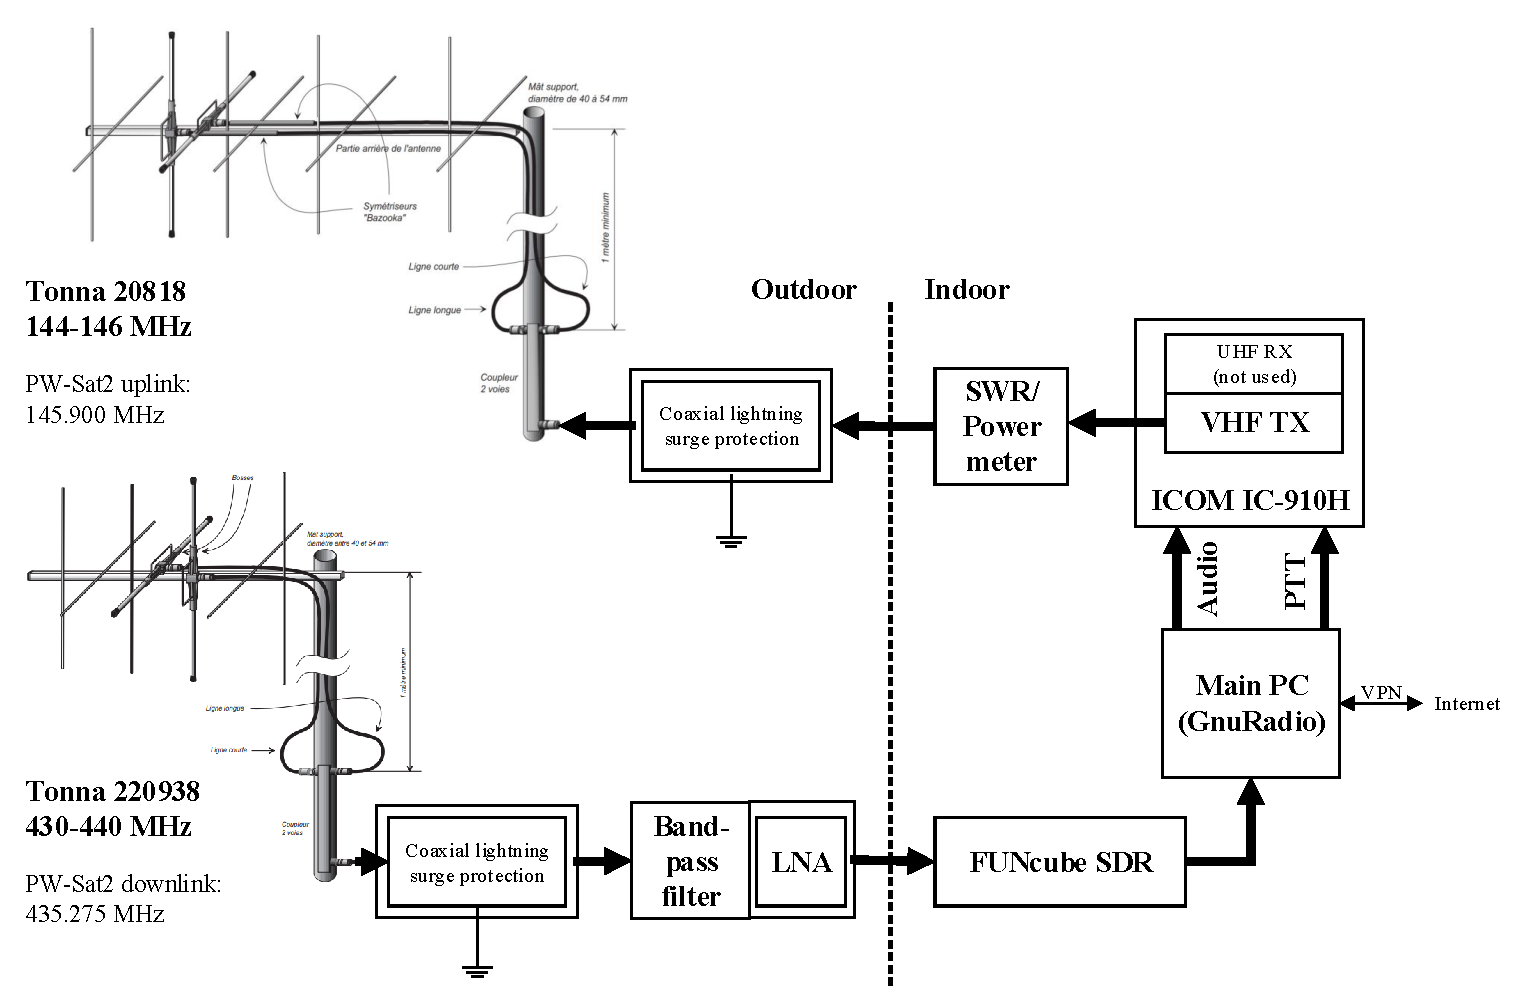
\includegraphics[width=0.8\paperwidth]{img/5/gs_block_diagram.eps}
    \caption{Ground station block diagram}
    \label{gs_block_diagram}
\end{figure}

\section{Antenna mast \& equipment}
Antenna mast \& rotator were already installed from previous experiments with satellite transmission. Main parameters: \SI{3}{\meter} height, SPID rotator with azimuth-elevator control. Mast with installed antennas is shown in the figure \ref{elka_antena_mast} and the antenna rotator is shown in the figure \ref{elka_antenna_rotator}.

\begin{figure}
    \centering
    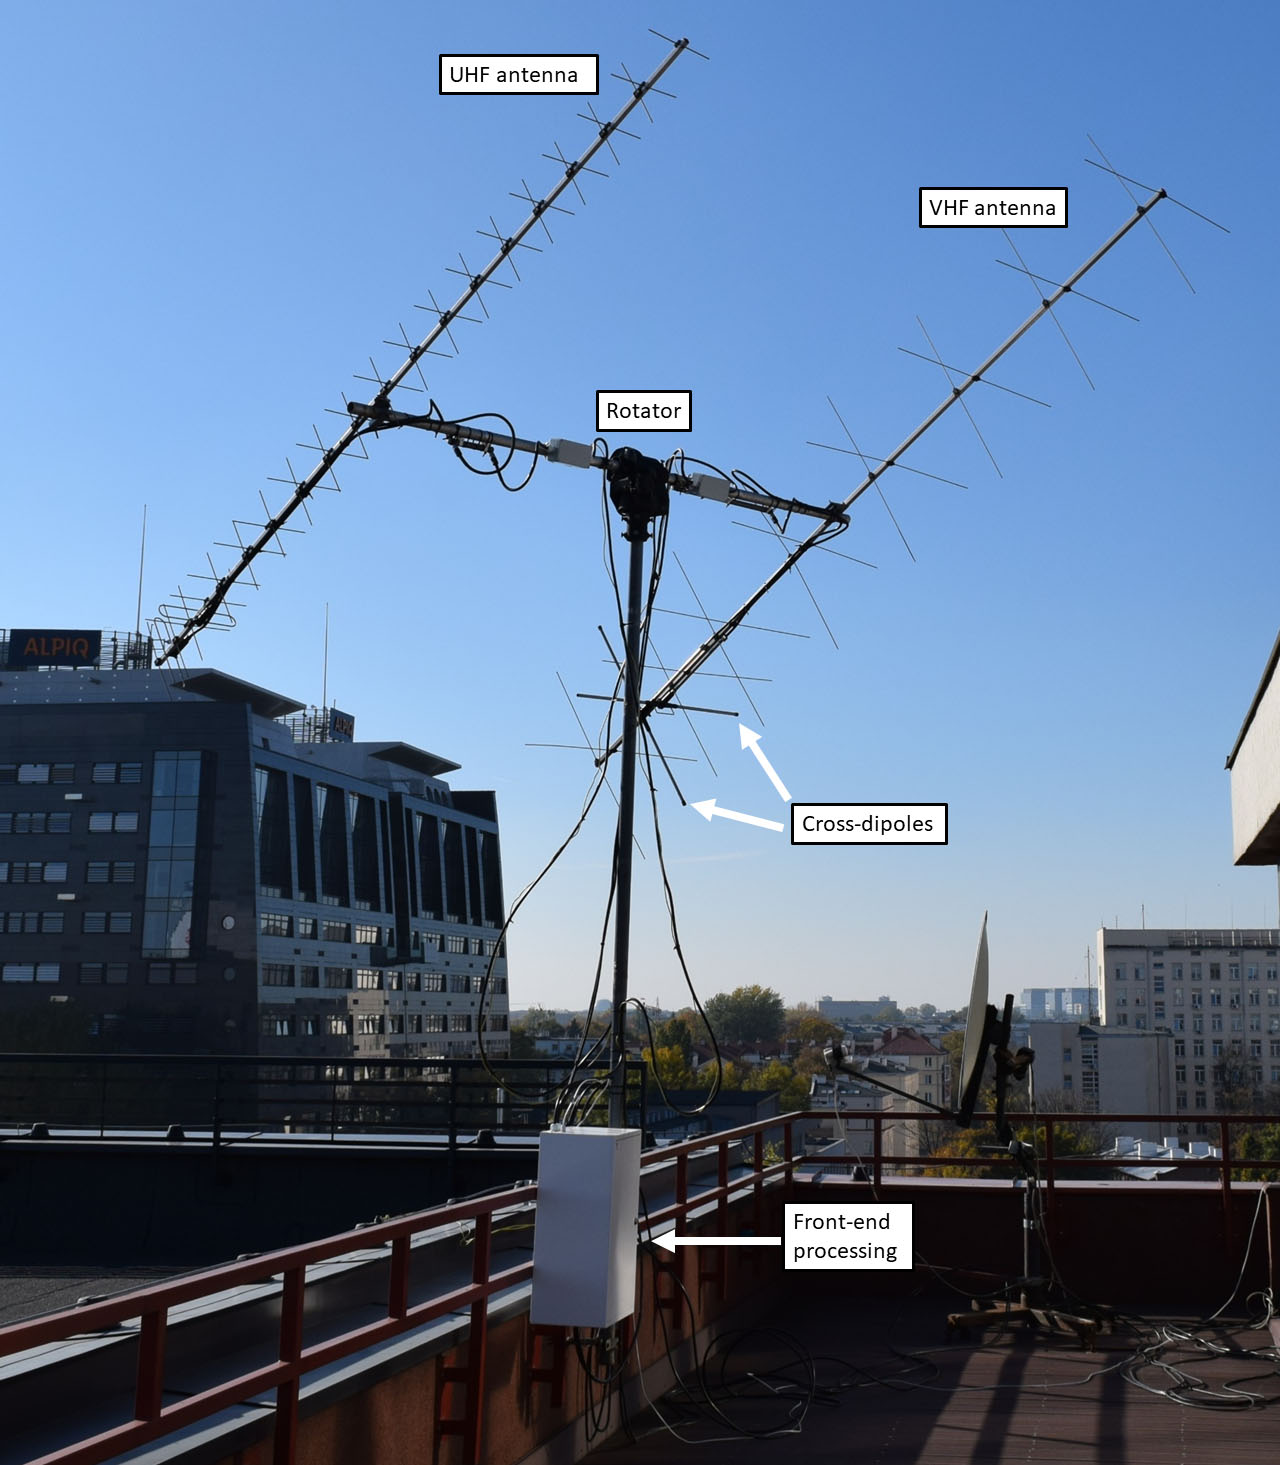
\includegraphics[width=0.5\paperwidth]{img/5/elka_antena_mast.jpg}
    \caption{Ground station picture}
    \label{elka_antena_mast}
\end{figure}

\begin{figure}
    \centering
    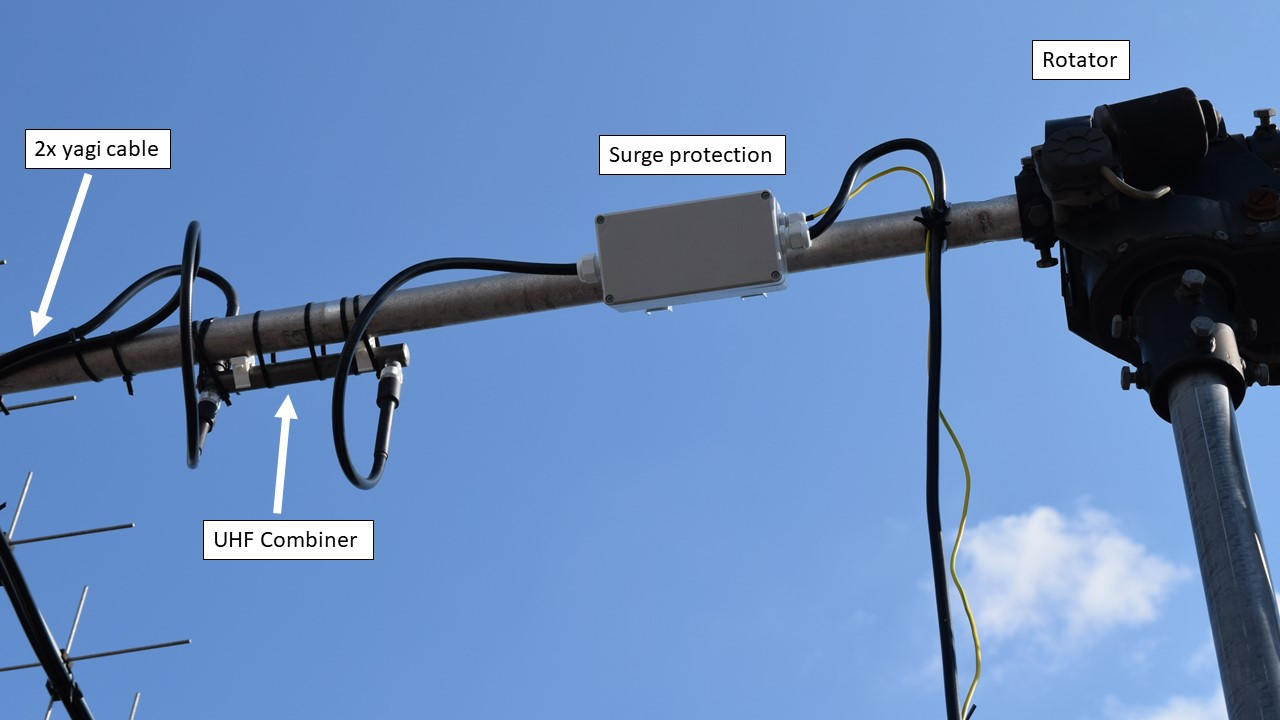
\includegraphics[width=0.75\paperwidth]{img/5/elka_antenna_rotator.jpg}
    \caption{Antenna rotator and boom}
    \label{elka_antenna_rotator}
\end{figure}

Coaxial lightning surge protector SP3000W installed on the mast is shown in the figure \ref{coax_surge_protection}. This elemnent discharges any high voltage pulses which can happen suring the lightning by the cost of insertion loss (declared \SI{0.2}{\dB}).

\begin{figure}
    \centering
    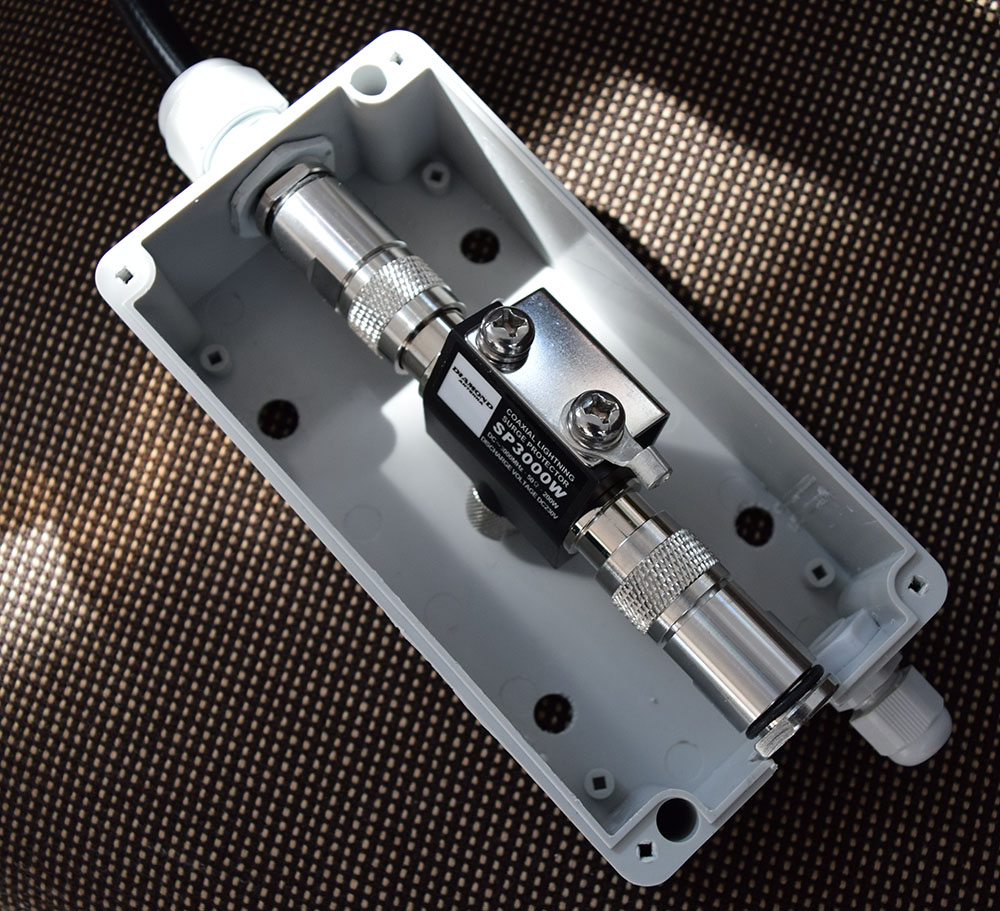
\includegraphics[width=0.5\paperwidth]{img/5/coax_surge_protection.jpg}
    \caption{Diamond SP3000W coaxial lightning surge protector}
    \label{coax_surge_protection}
\end{figure}



\section{Antennas}
PW-Sat2 is transmitting radio signals with linear polarization, nevertheless ground station  polarization should be circular, due to the random tumbling of the satellite. This will reduce the gain of the antennas, but the signal strength will be constant regardless of the satellite rotation. Cross-Yagi antennas were selected, and two linear planes antennas were phased with coaxial cable and symmetrical splitters/combiners. The diagram of the antenna phasing is shown in the figure \ref{antenna_phasing_diagram}. The length of the cables between the splitter/combiner and the dipoles should, with the dipole shift on the boom, create a \SI{90}{\degree} shift to create circular polarization. Two splitters/combiners were selected for antenna phasing: Tonna 31202 for VHF and Tonna 31270 for UHF.

\begin{figure}
    \centering
    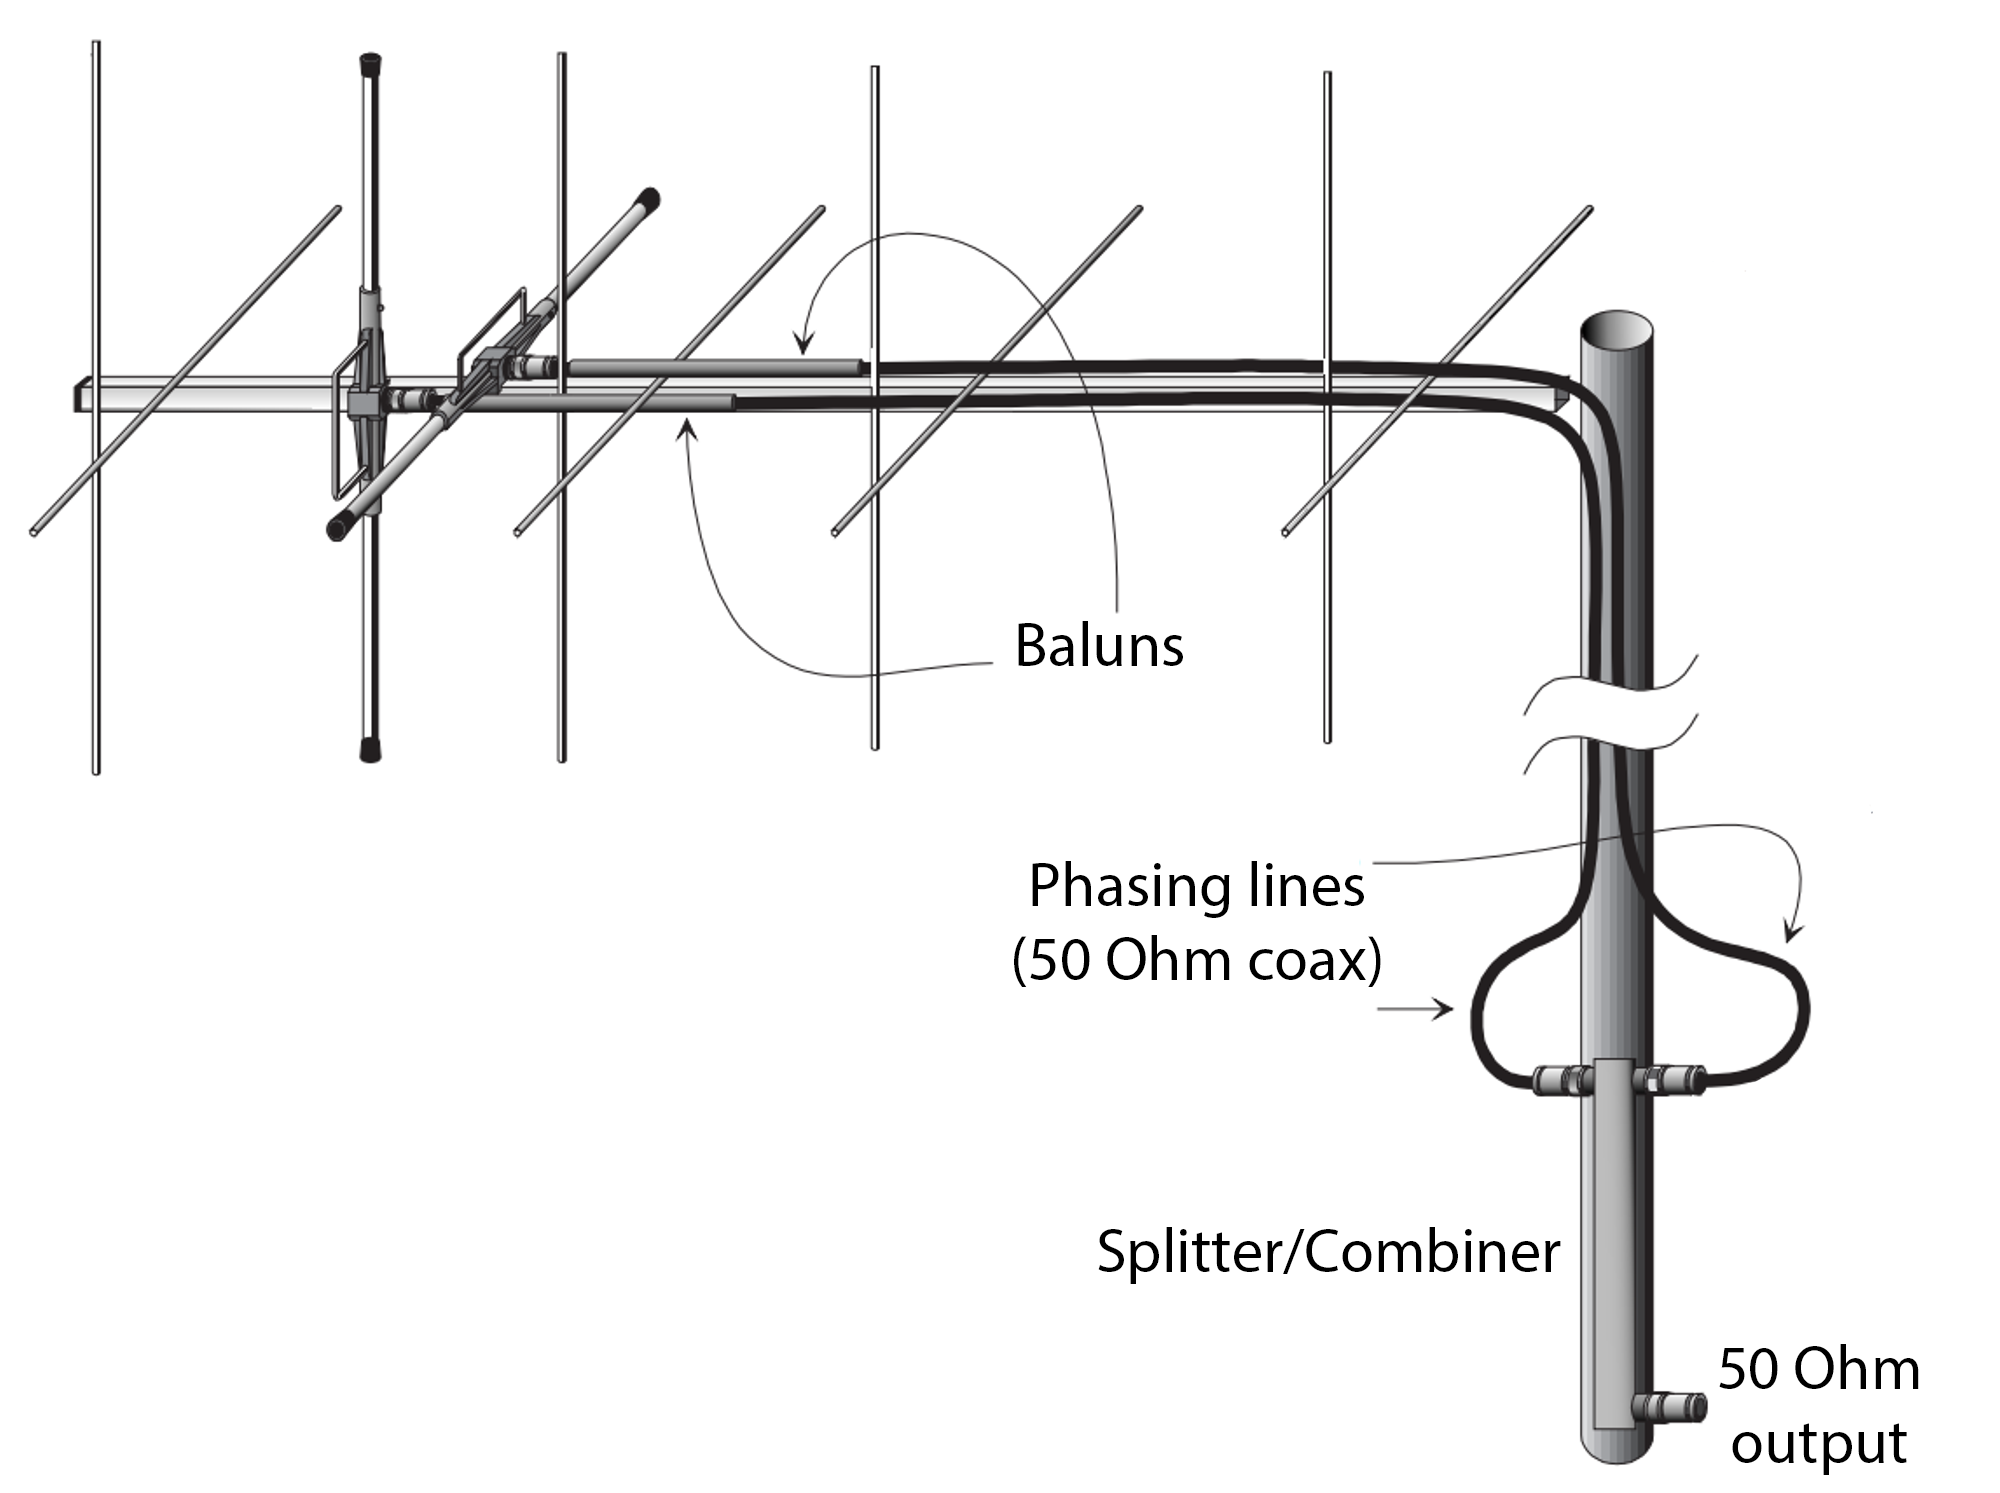
\includegraphics[width=0.5\paperwidth]{img/5/antenna_phasing_diagram.png}
    \caption{Antenna phasing}
    \label{antenna_phasing_diagram}
\end{figure}


Radiation patterns of the antennas are shown in the figures \ref{radiation_144} and \ref{radiation_435} as declared by the manufacturer.


Antennas were selected to be the longest possible, limited by the antenna mast height. Selected antenna characteristics:

\begin{tabular}{c|c}
     \textbf{Downlink} & \textbf{Uplink} \\ \hline
     Tonna 220938 & Tonna 20818 \\
     UHF 2x 19 elements & VHF 2x 9 elements \\
     loop dipole & linear dipole \\
     \SI{16.2}{\dBi} gain & \SI{13.2}{\dBi} gain \\
     \SI{30}{\degree} beamwidth & \SI{40}{\degree} beamwidth
\end{tabular}

\begin{figure}
    \centering
    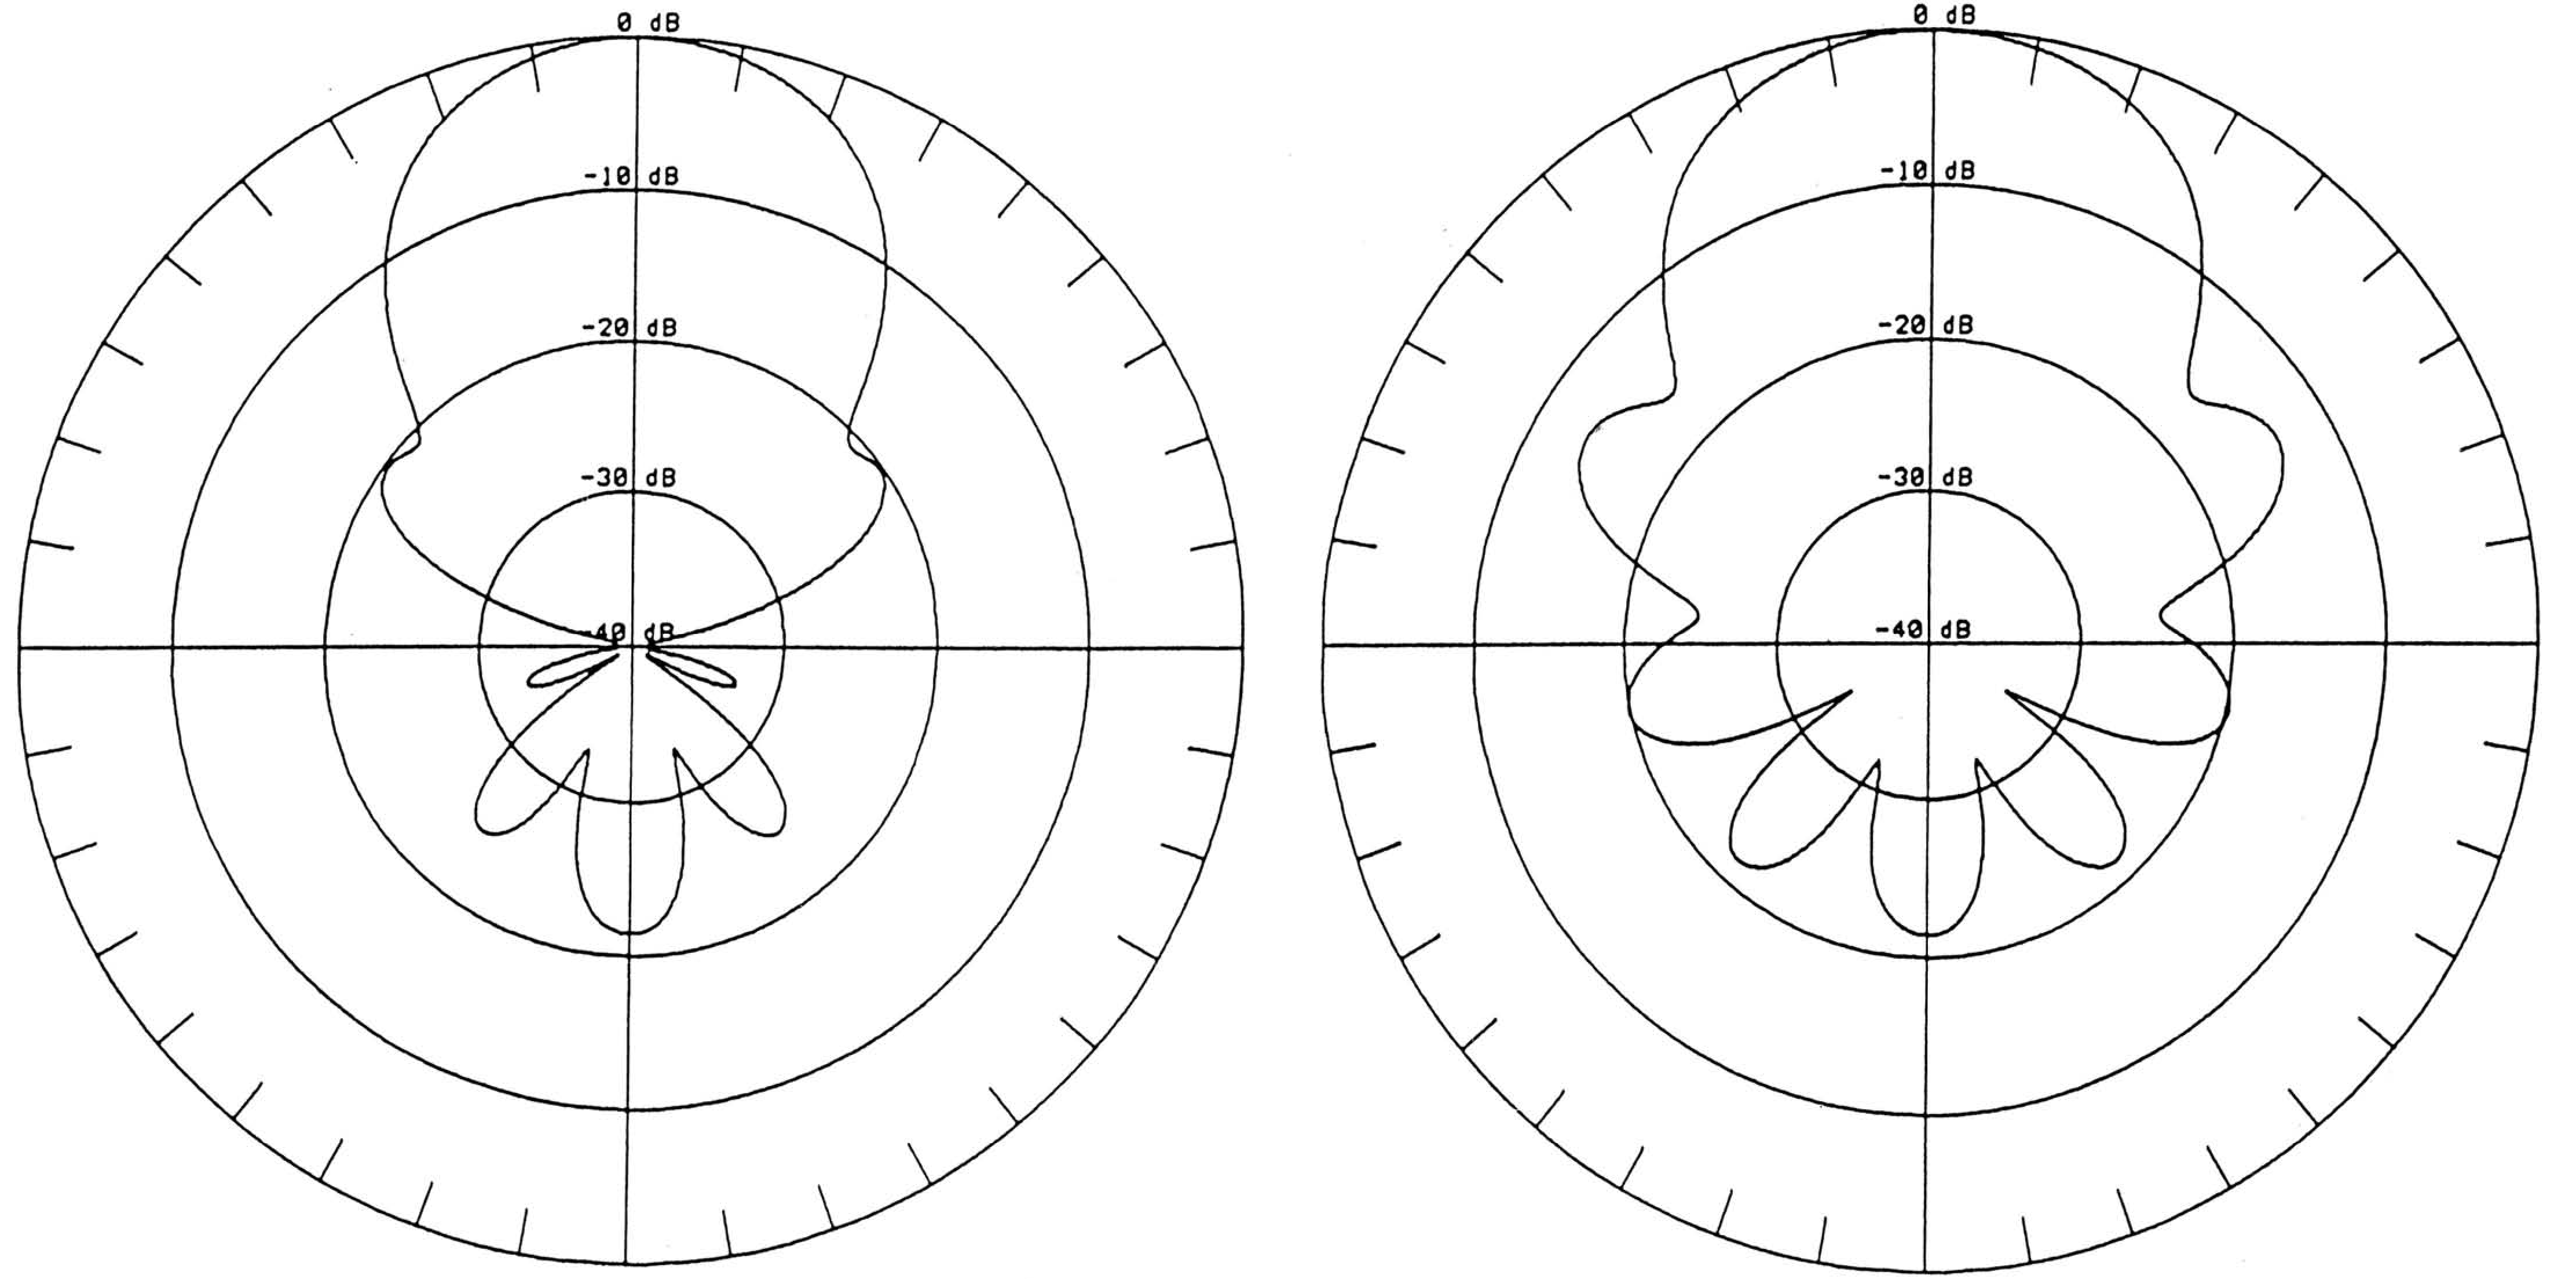
\includegraphics[width=0.75\paperwidth]{img/5/radiation_144.png}
    \caption{VHF antenna radiation patter - E and H plane.}
    \label{radiation_144}
\end{figure}

\begin{figure}
    \centering
    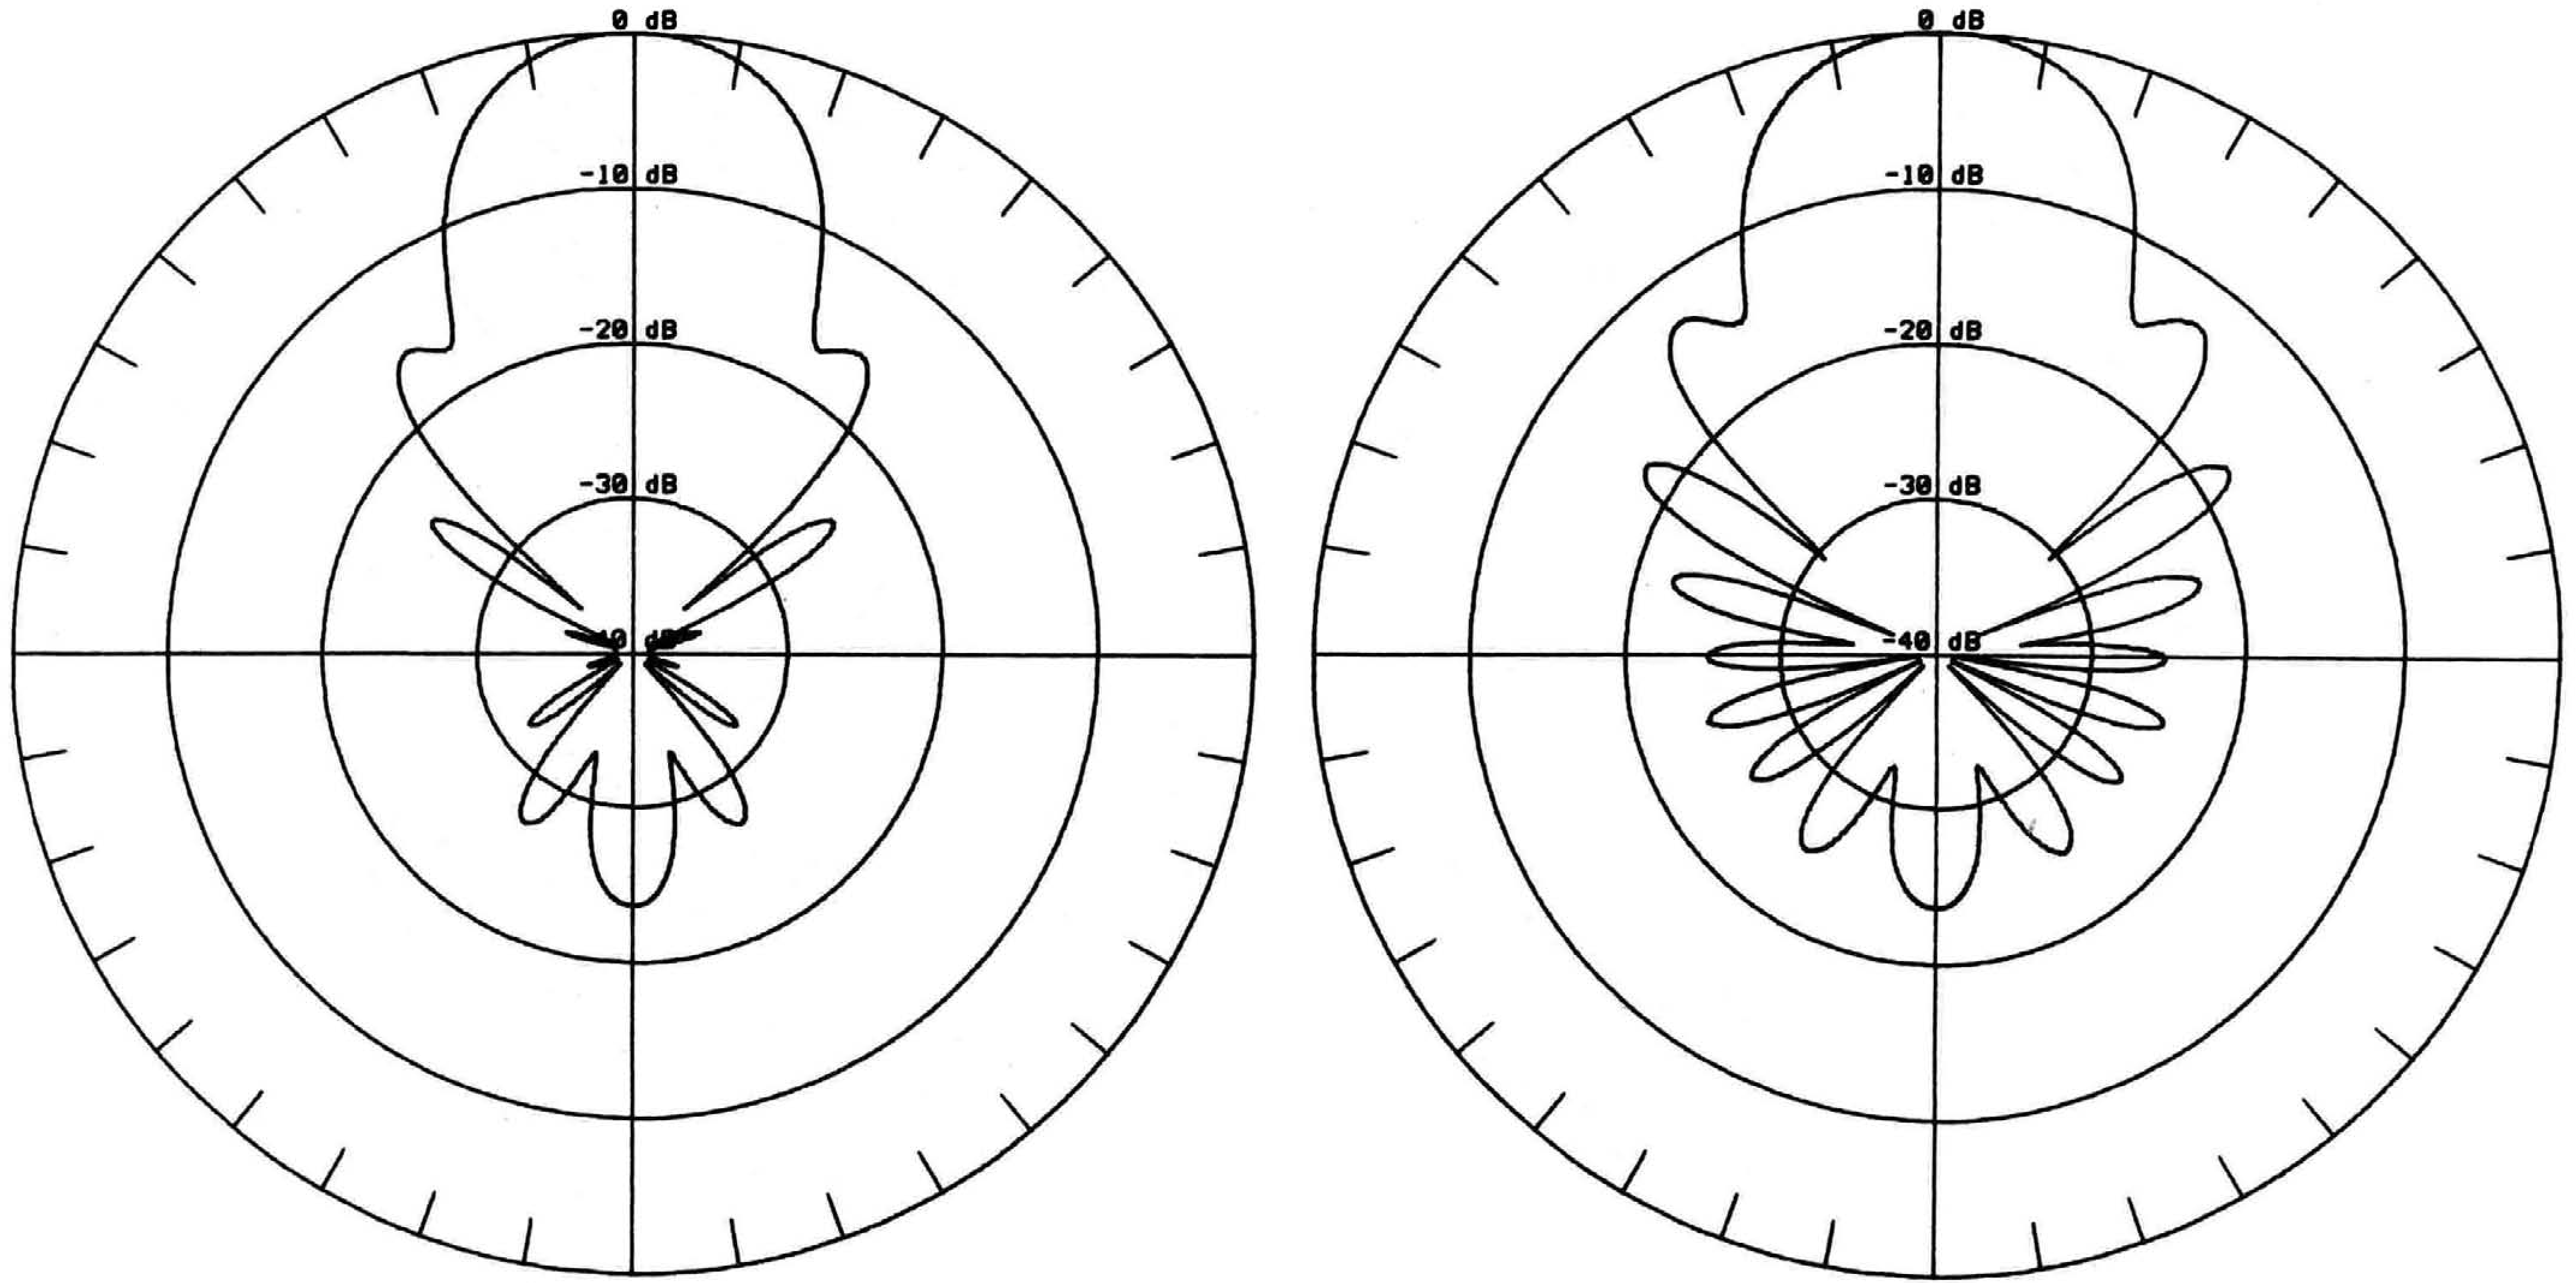
\includegraphics[width=0.75\paperwidth]{img/5/radiation_435.png}
    \caption{UHF antenna radiation patter - E and H plane.}
    \label{radiation_435}
\end{figure}



\subsection{Splitters/combiners measurements}
Splitters/combiners were tested prior to its mounting. The most important parameters of the splitter is the insertion loss, amplitude and phase imbalance between the paths and the isolation of the splitter. All of the parameters were tested using Rohde \& Schwarz ZVL Vector Network Analyser, in the configurations shown in the figure \ref{splitter_measurement_diagram}. The results of the insertion loss (Fig. \ref{splitter_amplitude}) show that it is negligible - unmeasurable within tolerances of the VNA. Amplitude imbalance is also very good - much less than \SI{0.1}{\dB}. The phase imbalance is also very good for both splitters (Fig. \ref{splitter_phase}) - less than \SI{1}{\degree}. The isolation (Fig. \ref{splitter_isolation}) is the worst parameter of the measured splitters (only about \SI{6}{\dB}), but in the case when both antennas work together it is not an issue.

\begin{figure}
    \centering
    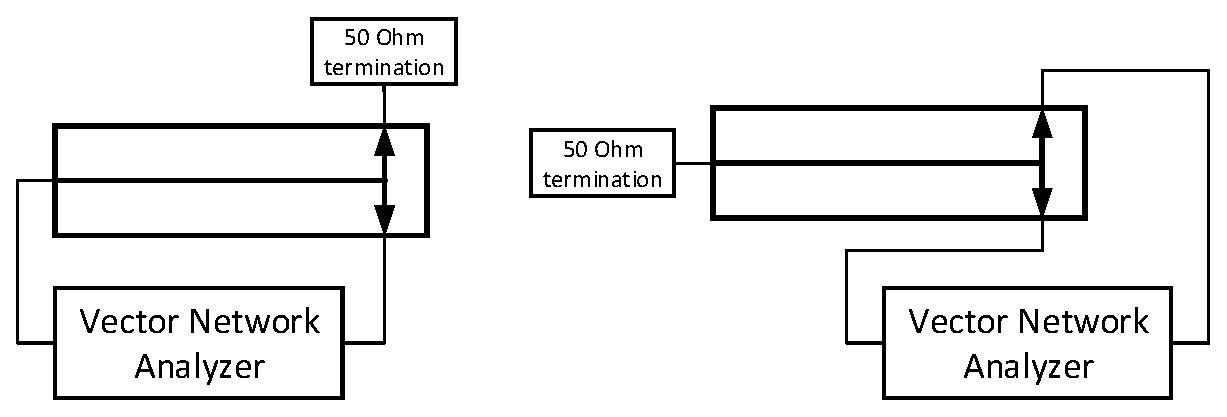
\includegraphics[width=0.75\paperwidth]{img/5/splitter_measurement_diagram.eps}
    \caption{Splitter/combiner measurement block diagram for through and isolation measurement}
    \label{splitter_measurement_diagram}
\end{figure}

\begin{figure}
    \centering
    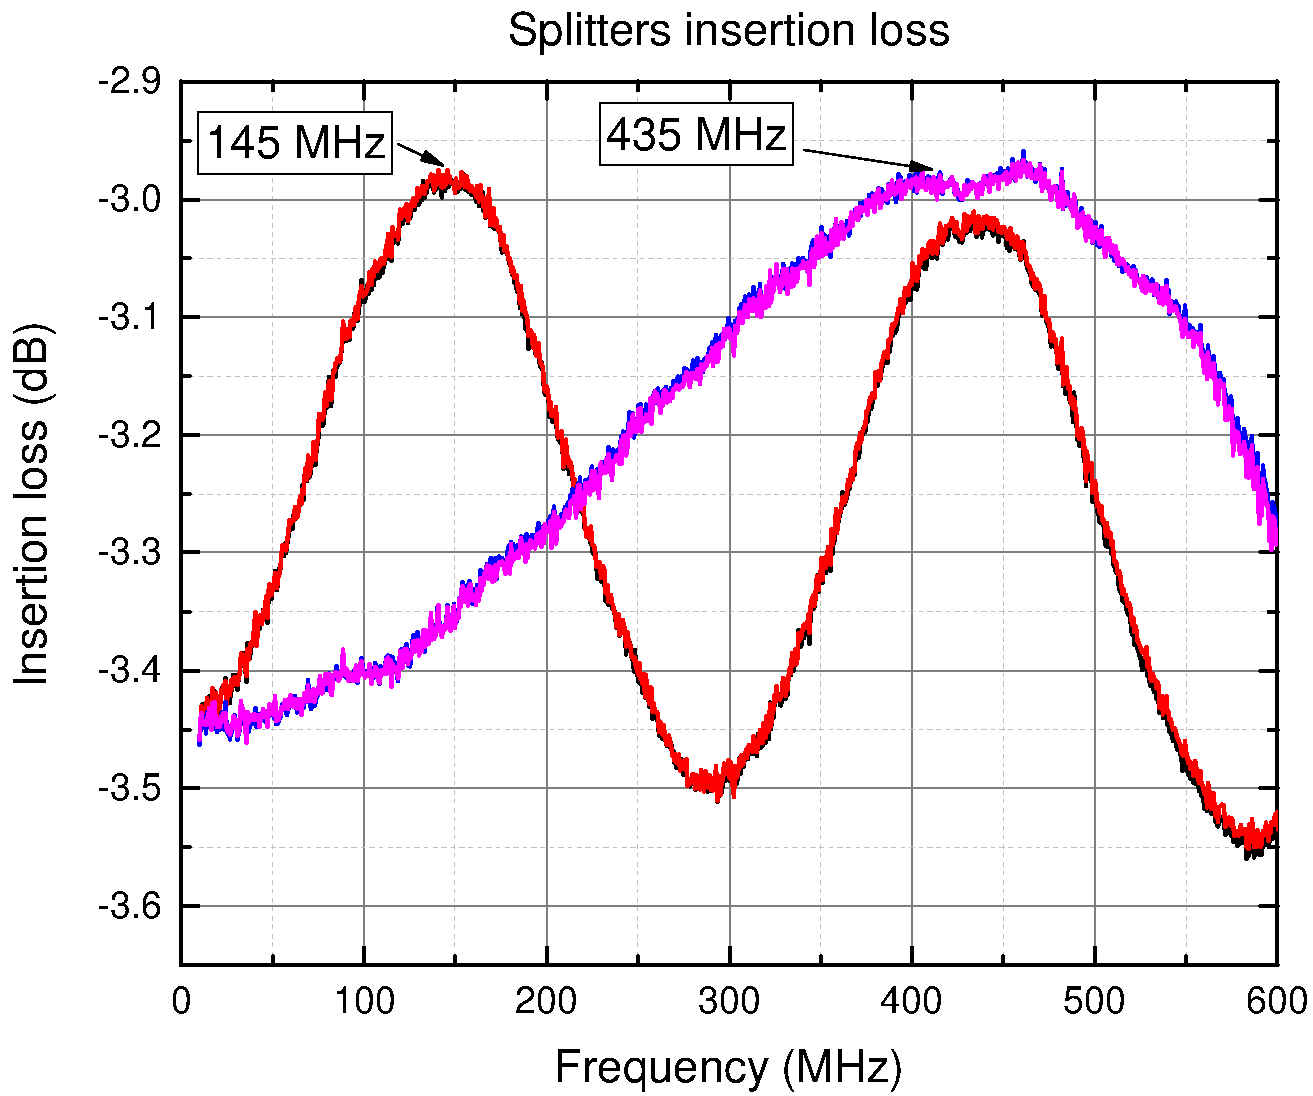
\includegraphics[width=0.6\paperwidth]{img/5/splitter_amplitude.pdf}
    \caption{Splitters/combiners insertion loss}
    \label{splitter_amplitude}
\end{figure}

\begin{figure}
    \centering
    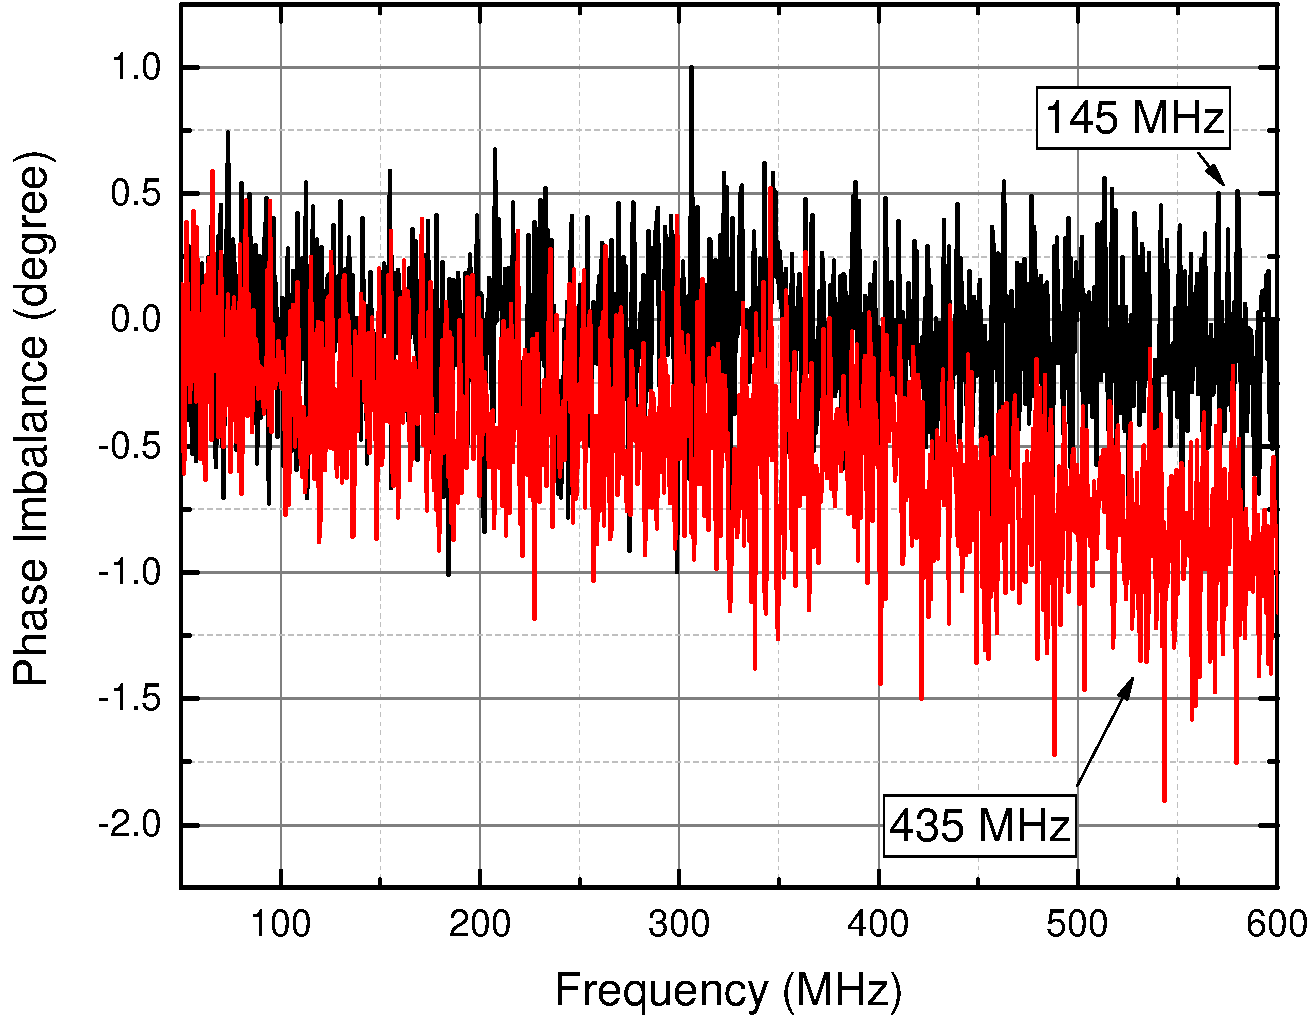
\includegraphics[width=0.6\paperwidth]{img/5/splitter_phase.pdf}
    \caption{Splitters/combiners phase shift imbalance}
    \label{splitter_phase}
\end{figure}

\begin{figure}
    \centering
    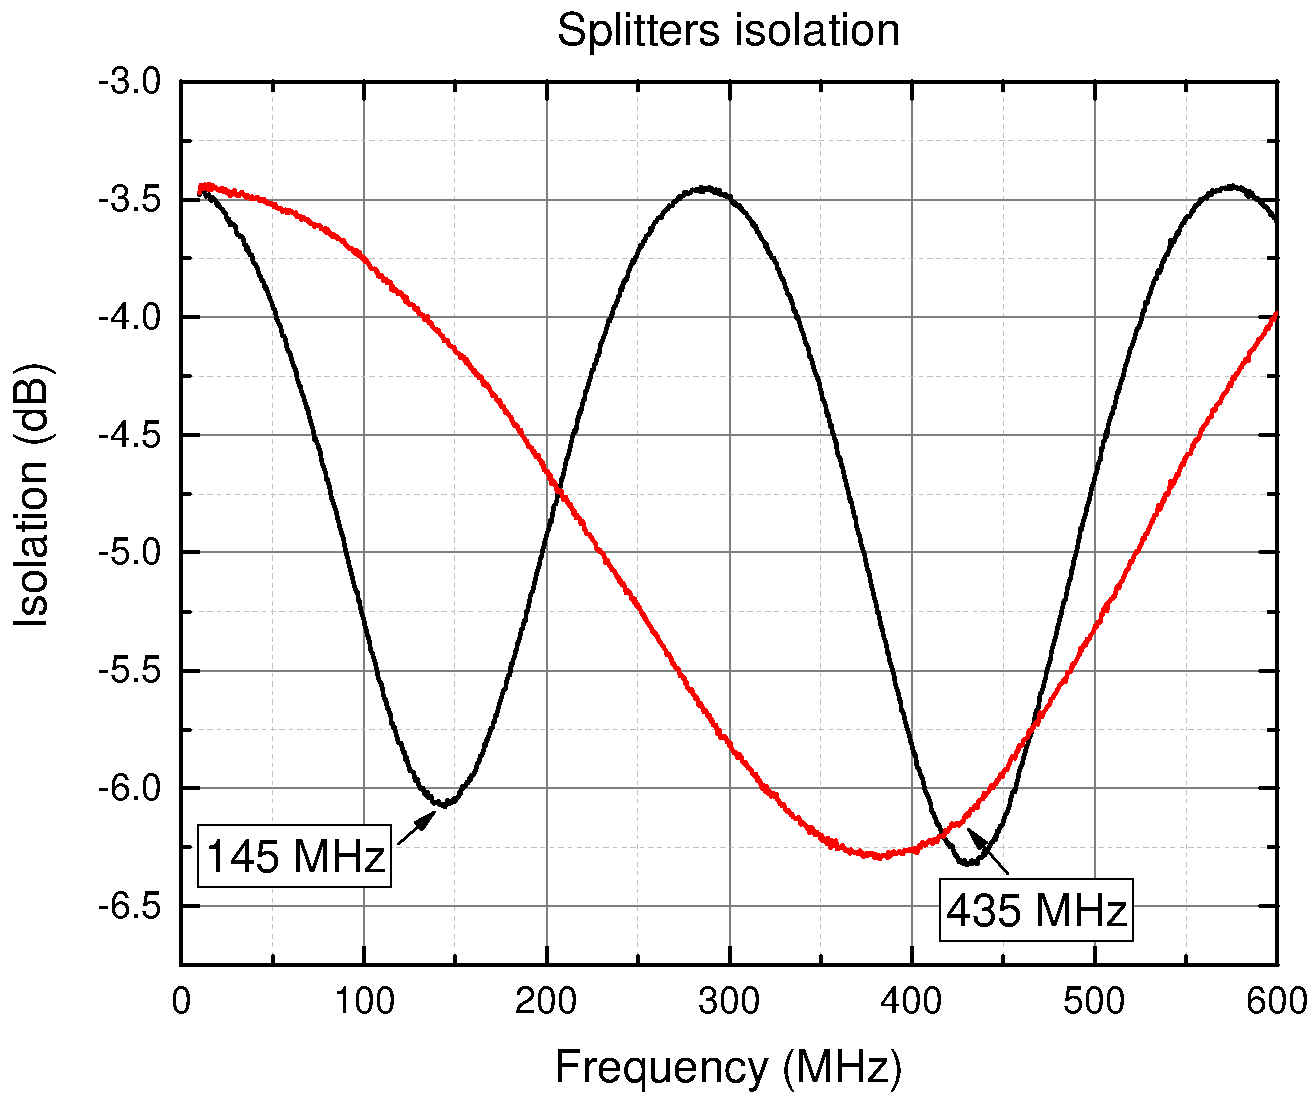
\includegraphics[width=0.6\paperwidth]{img/5/splitter_isolation.pdf}
    \caption{Splitters/combiners isolation}
    \label{splitter_isolation}
\end{figure}


\subsection{Antenna Measurements}
After the assembly, antennas were measured for their impedance matching and resonance. As the antennas are Yagi-Uda type, the most important element for matching is the dipole itself. Each antenna consist of two dipoles (with vertical and horizontal polarization) phased with a combiner. Measurements of the dipoles and the phased antenna were performed, and the result is shown in the table \ref{TODO}.


\section{Uplink data flow}
Block diagram of uplink data chain is shown in the figure \ref{uplink_data_flow}. The telecommands issued by the operator are converted to the radio frames (\textbf{0}s and \textbf{1}s bits), later FSK modulated using GNUradio, finally to be FM-modulated, up-converted and power amplified by conventional voice transceiver.

\begin{figure}
    \centering
    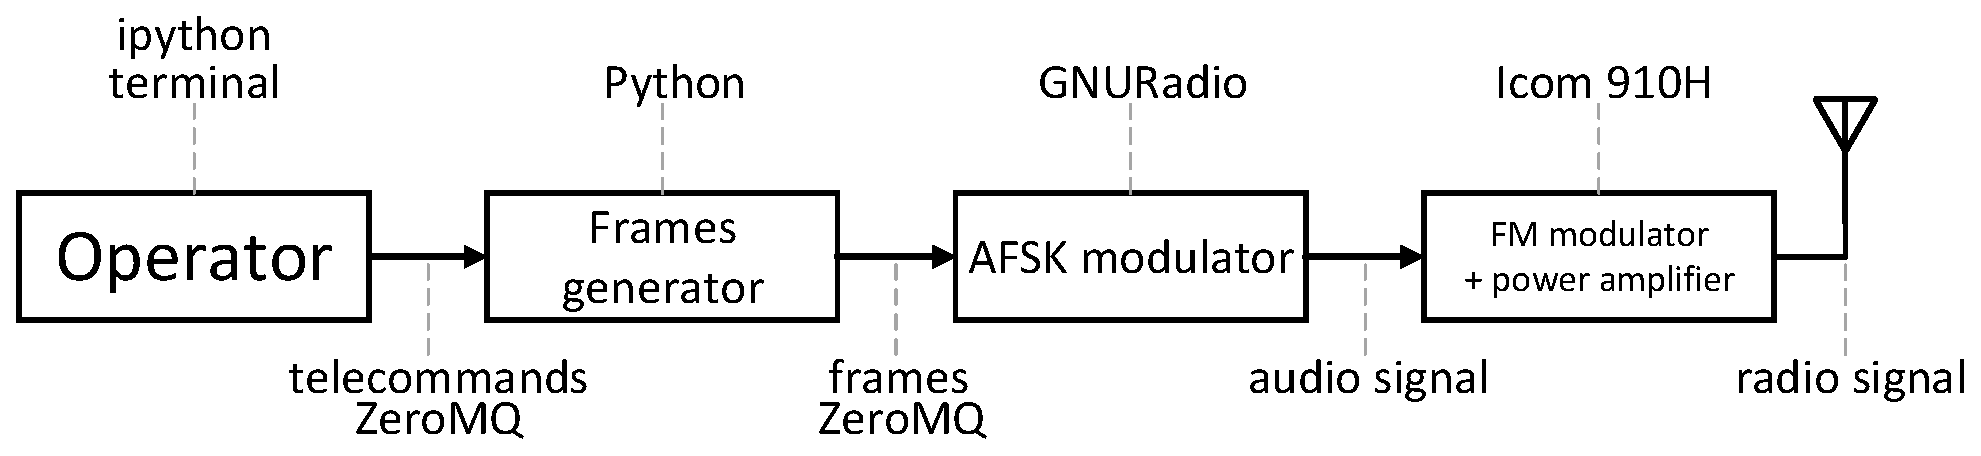
\includegraphics[width=0.6\paperwidth]{img/5/uplink_data_flow.eps}
    \caption{Uplink data flow}
    \label{uplink_data_flow}
\end{figure}

\section{Uplink baseband generation}
AFSK signal is generated by the GNURadio flowgraph shown in the figure \ref{uplink_flowgraph}. First, the telecommand is received by ZeroMQ slot, the packet is formatted and is is changed to the stream of bits. Each bit of the signal controls the frequency of the Voltage Controlled Oscillator (VCO) (\SI{1200}{\hertz} or \SI{2200}{\hertz} for \textbf{0} and \textbf{1}, respectively). During packet transmission, the transmit signal of the radio is enabled, and the audio signal is then generated by the audio card.

\begin{figure}
    \centering
    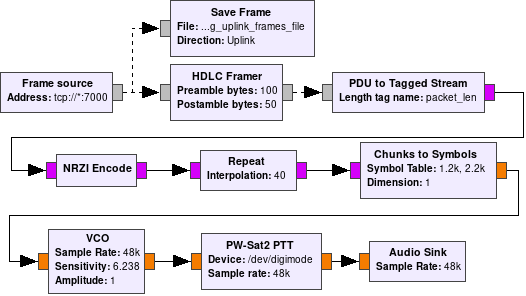
\includegraphics[width=0.8\paperwidth]{img/5/uplink_flowgraph.png}
    \caption{Uplink GNURadio companion flowchart}
    \label{uplink_flowgraph}
\end{figure}


\section{Uplink - transmitter}
Analog audio FM transceiver can be used to generate RF signal. The frequency deviation of the modulation was selected to allow to use radio amateur voice transceivers. Audio FSK signal (before FM-modulation) is generated by the software running on the PC. Radio is connected to the computer, which controls the audio to transmit and Push-To-Talk (PTT, transmission enable) signal.

During PW-Sat1 project, the Icom 910H amateur radio transceiver was used for both uplink and downlink, therefore it was proposed to use the the same radio as it do comply with all the requirements. Radio is shown in the figure \ref{Icom_910H_ref}. In case or need of larger output power the high-power amplifier can be connected to the output of the radio.

\begin{figure}
    \centering
    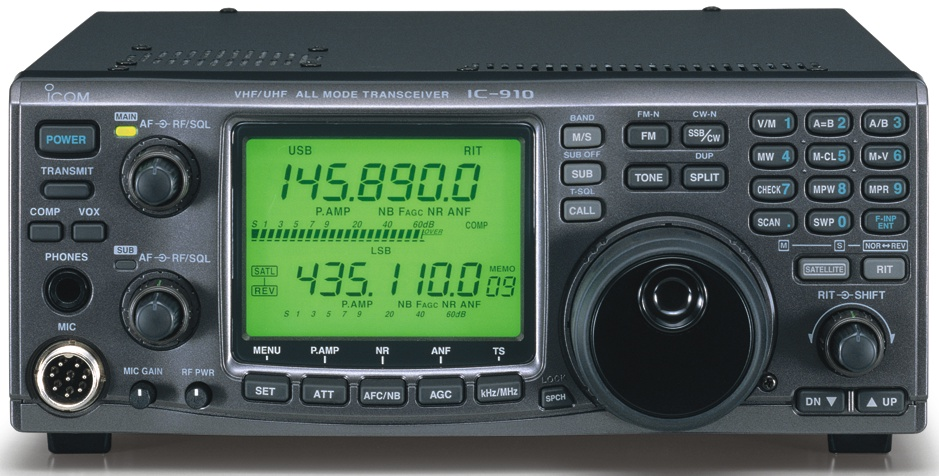
\includegraphics[width=0.6\paperwidth]{img/5/icom910h.jpg}
    \caption{Icom 910H. Source: \cite{ICOM_910H_pic}}
    \label{Icom_910H_ref}
\end{figure}

Radio VHF FM transmit characteristics:

\begin{tabular}{c|c}
    Frequency & \si{144} - \SI{148}{\MHz} \\
    Frequency stability &  \SI{\pm 3}{\ppm} \\
    Output power & \SI{100}{\watt} \\
    Audio input & analog jack \\
    Audio bandwidth & \SI{4}{\kHz} \\
\end{tabular}

\subsection{Standing Wave Ratio meter}
To check proper antenna connection and ensure long-term monitoring a SWR (Standing Wave Ratio) was installed. This instrument measures ratio of reflected power, thus providing information about antenna impedance matching. In case of antenna cracks or bending due to the high wind, any anomalies in the matching can be detected. SWR meter during the transmission is shown in the figure \ref{swr_meter_photo}, indicating that the VSWR of the antennas is lower than \si{1.05}. The output power is measured along the VSWR, and during the transmission it was equal to \SI{80}{\watt}.

\begin{figure}
    \centering
    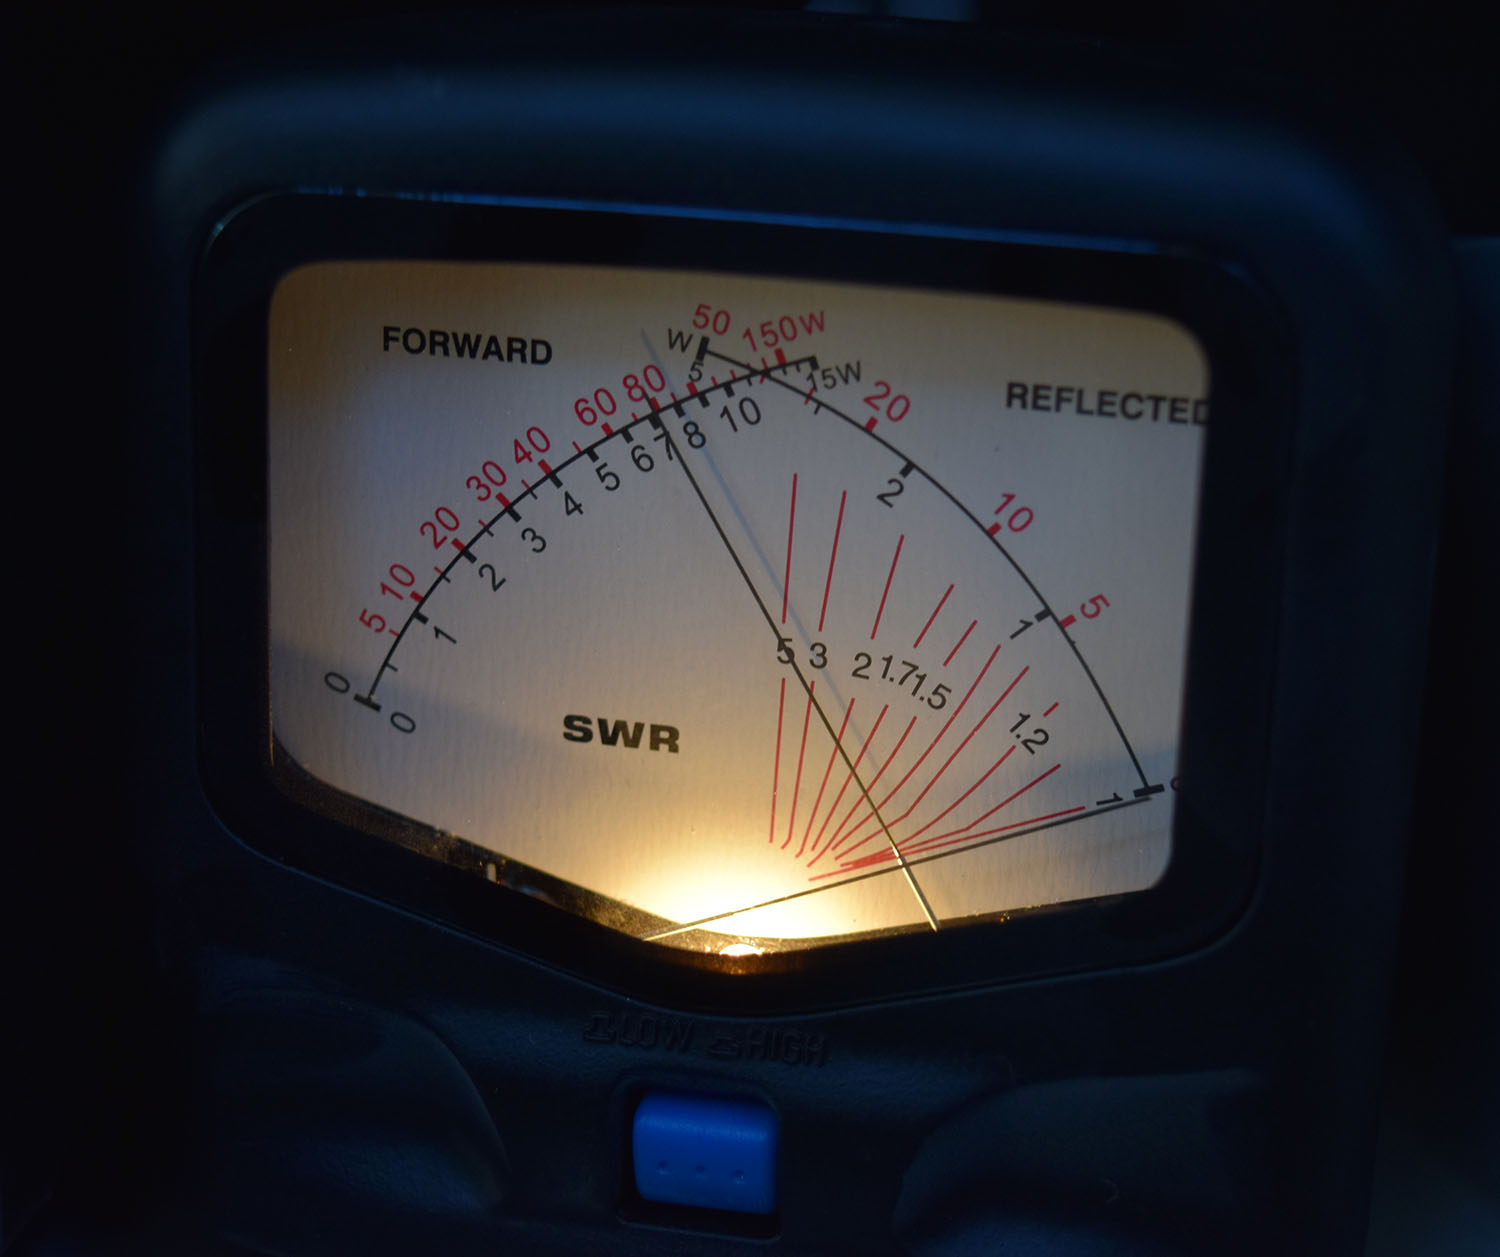
\includegraphics[width=0.6\paperwidth]{img/5/swr_meter_photo.jpg}
    \caption{Standing Wave Ratio meter during transmission}
    \label{swr_meter_photo}
\end{figure}


% \subsection{Measurements}
% As the uplink was built using conventional HAM radio transceiver, only the modulation and output power should be measured. As the physical layer is the typical FM-modulated AFSK and frame protocol is typical AX.25 there is a lot of free software to verify the correctness of the frame and modulation.

\subsubsection{Spectrum \& Watchdogs}
The spectrum and output modulation correctness in constantly monitored using so-called watchdog built using another Software Defined Radios (PlutoSDR, RTL-SDR) placed in the proximity of the main antennas.
By demodulating uplink signal and comparing it in the real time with transmitted frames the correctness of the transmission is guaranteed. Watchdog flowchart and graphical view are shown in the figure \ref{uplink_watchdog_flowgraph}.

\begin{figure}
    \centering
    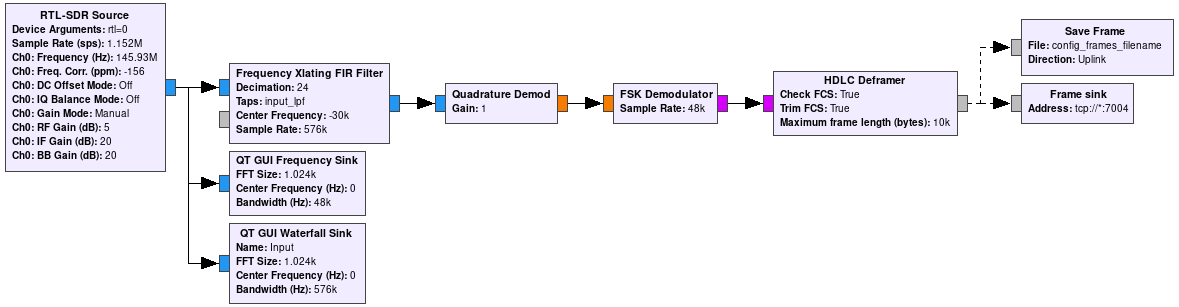
\includegraphics[width=0.8\paperwidth]{img/5/uplink_watchdog_flowgraph.png}
    \caption{Uplink watchdog GNURadio flowgraph}
    \label{uplink_watchdog_flowgraph}
\end{figure}


% ------------------------------------------------------------
% ------------------------- DOWNLINK -------------------------
% ------------------------------------------------------------

\section{Downlink}
Receiving Signals from maximal slant range of about \SI{3000}{\kilo\meter} from a \SI{0.5}{\watt} transmitter requires very high processing gain and low noise factor of the system. System also needs to compensate for Doppler effect and ground interferences. The block diagram of the signal flow is shown in the figure \ref{downlink_diagram}.

\begin{figure}
    \centering
    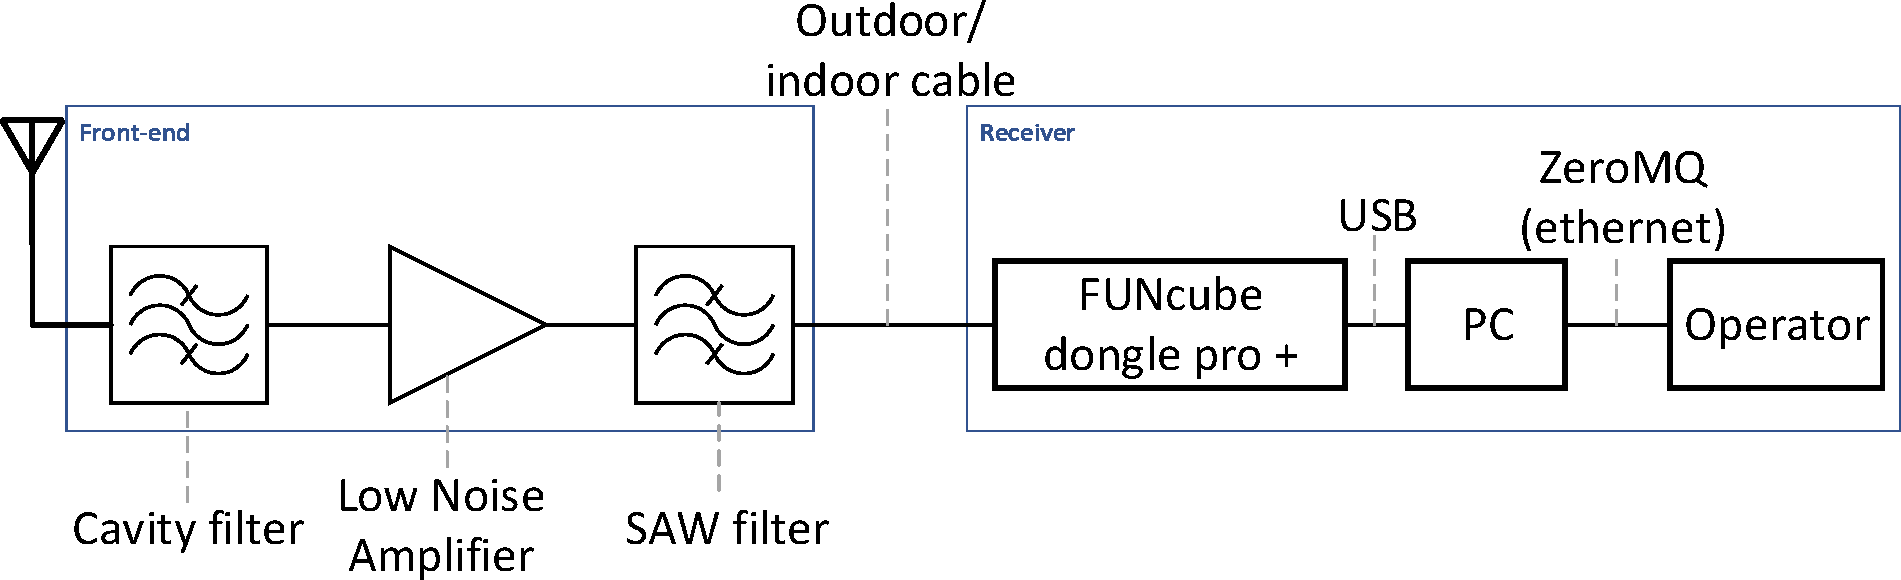
\includegraphics[width=0.8\paperwidth]{img/5/downlink_diagram.pdf}
    \caption{Downlink diagram}
    \label{downlink_diagram}
\end{figure}

\section{Signal front-end processing}
Radio front-end has two main purposes - to lower the system noise figure (by amplifying the signal with Low Noise Amplifier) and eliminate intermodulation with another signals (filtering). Its design consists of three stages: low loss cavity pass band filter, low noise amplifier and pass band SAW filter. 

Front-end signal processing is installed as close to the antenna as possible as shown in the figure \ref{elka_skrzynka}.

\begin{figure*}
   \centering
\begin{tabular}{cc}
        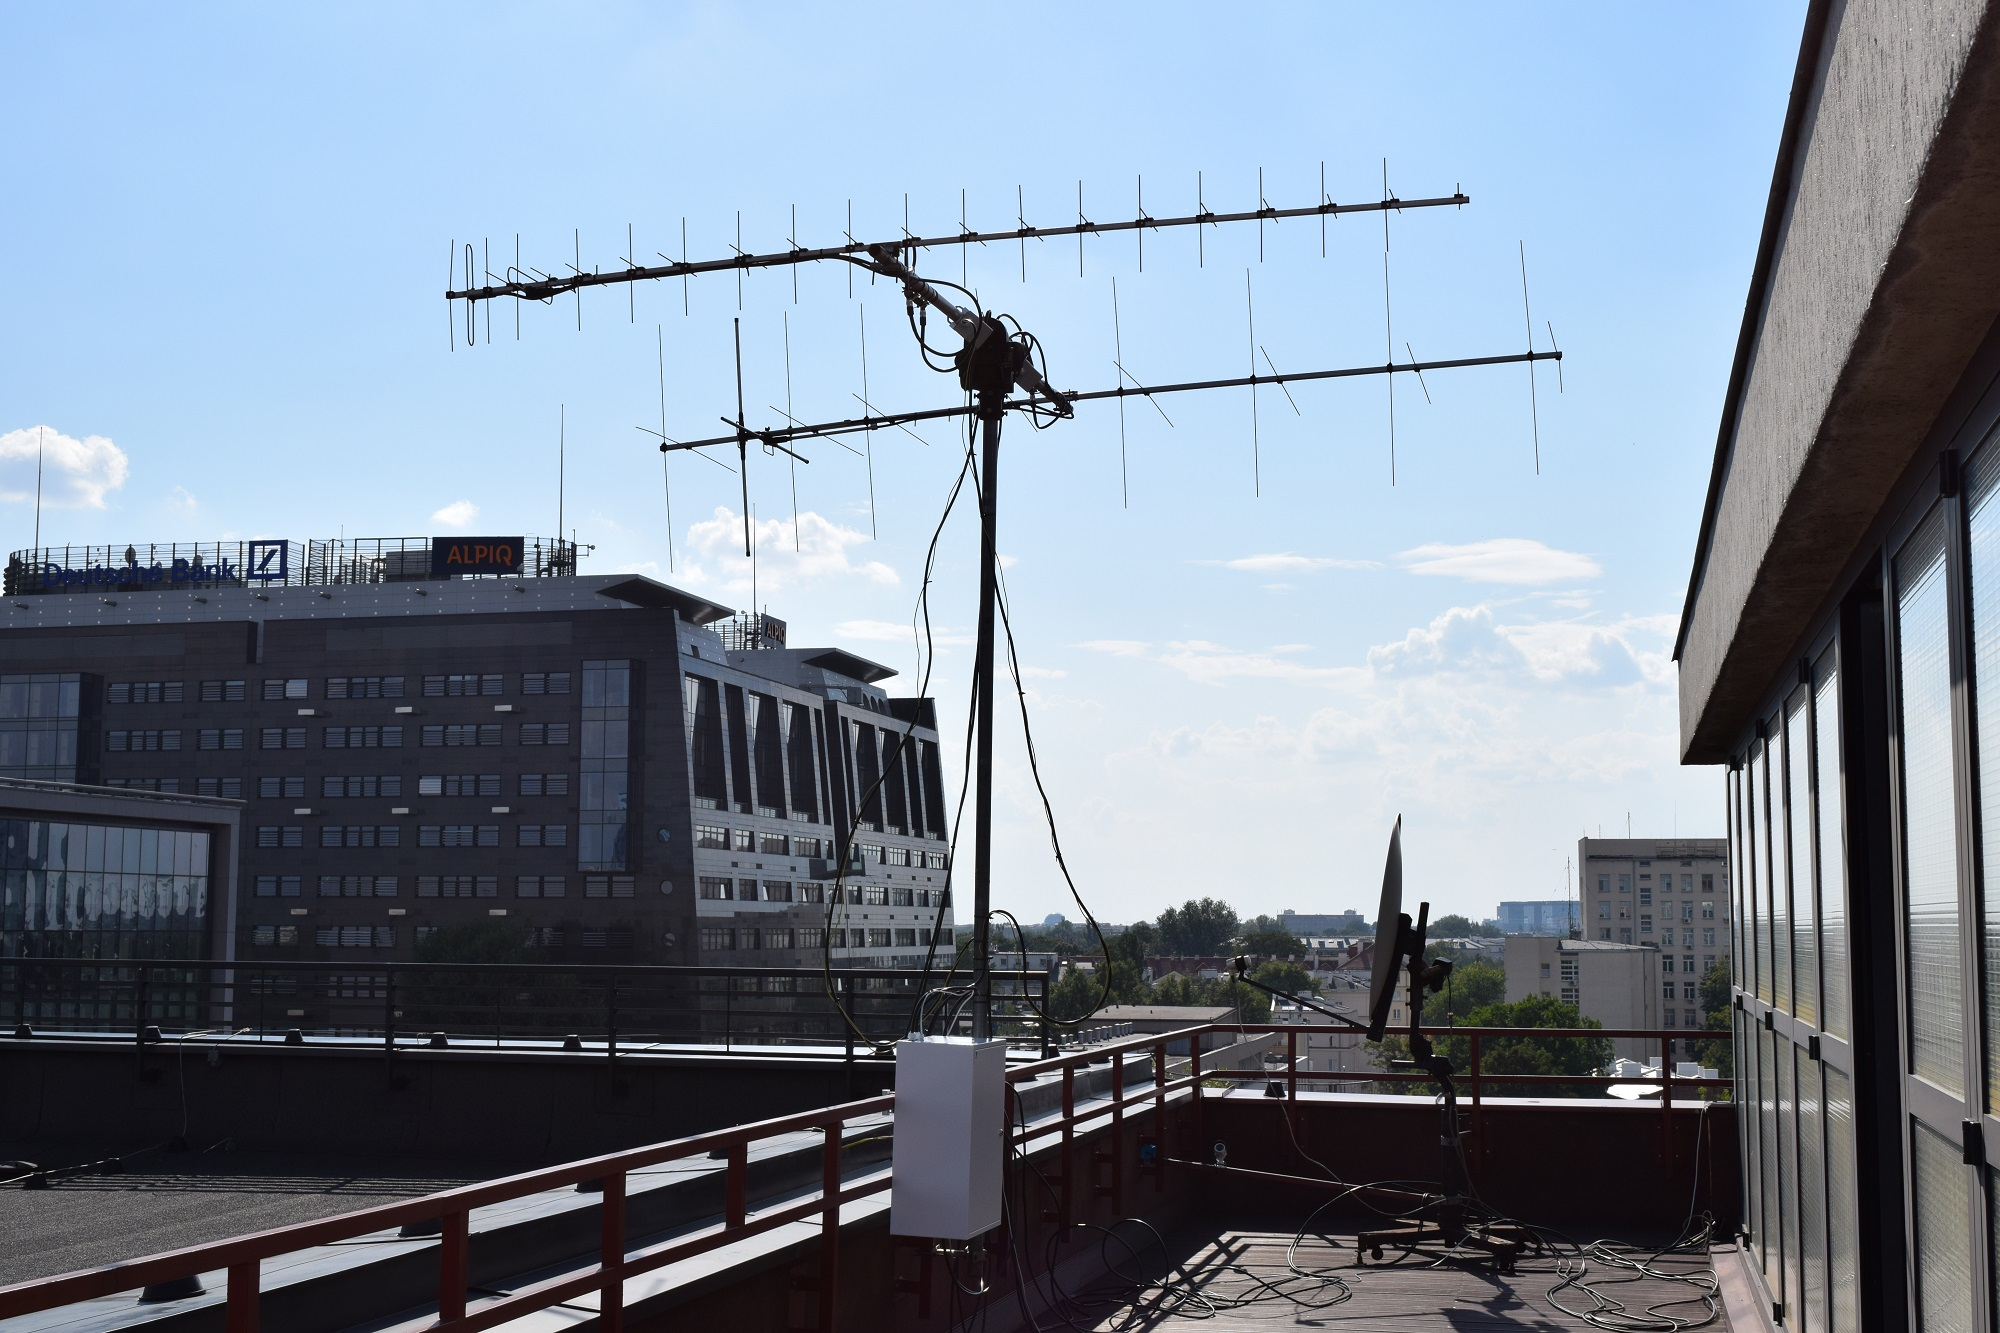
\includegraphics[width=0.3\paperwidth]{img/5/elka_view.jpg}
    & 
        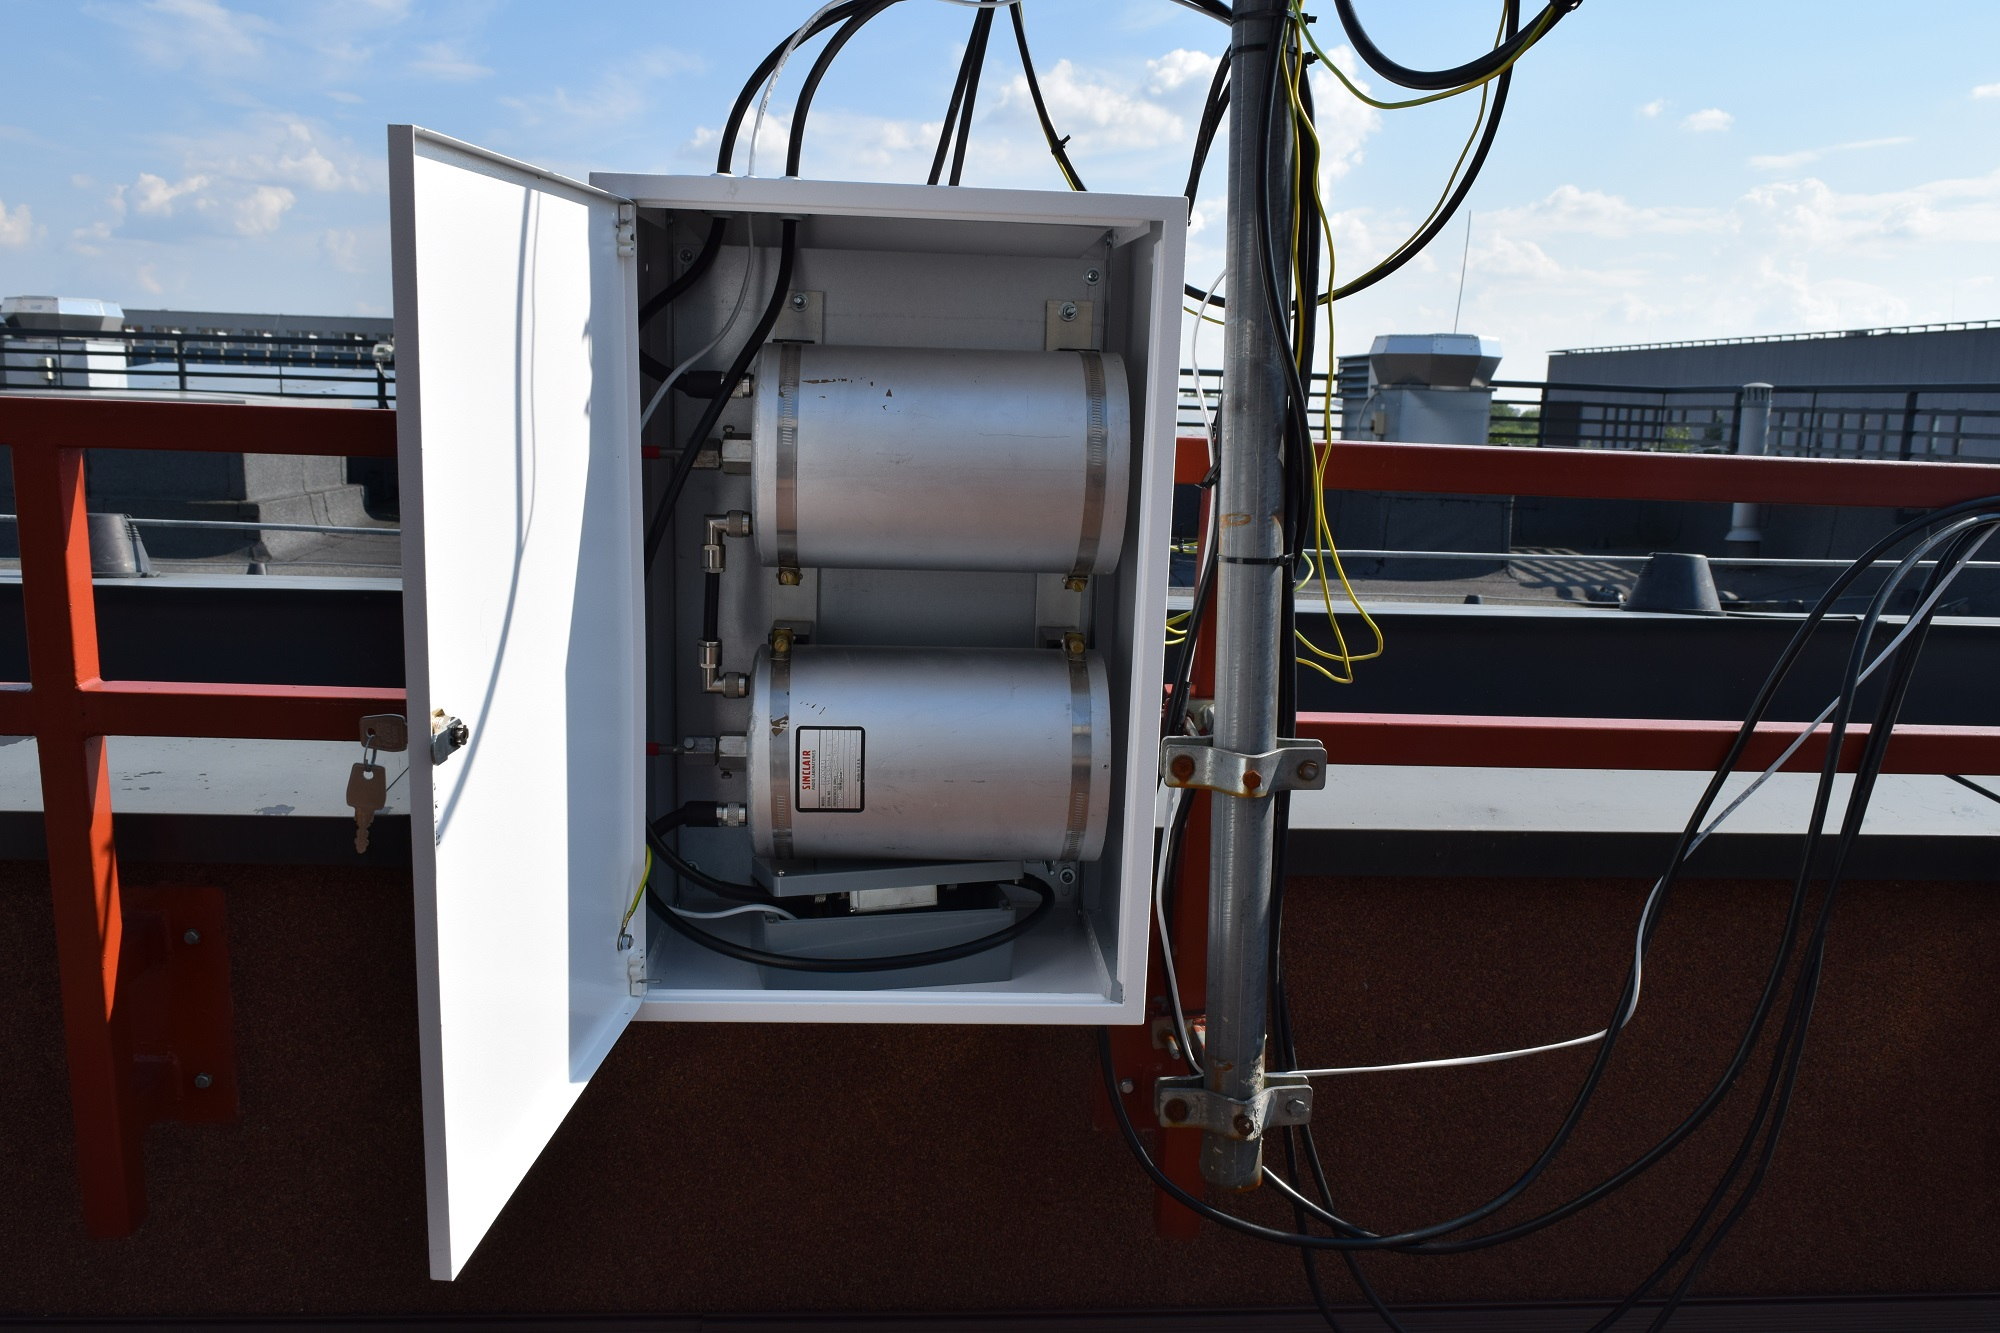
\includegraphics[width=0.3\paperwidth]{img/5/elka_skrzynka.jpg}
\end{tabular}
\label{elka_skrzynka}
\caption{PW-Sat2 ground station view and front-end processing.}
\end{figure*}

\subsection{Cavity filter}
Strong signals in the band of the amplifier can intermodulate, resulting in variety of issues: from reduced gain to completely distorted signal. Narrow-band cavity filter installed before the LNA to filter out out-of-band signals. Cavity filter due to its construction has very low insertion loss and regulated, narrow pass bandwidth in the cost of filter size and weight. Filter, shown in the figure \ref{cavity_filter_during_tuning} was tuned to the frequency of the PW-Sat2, with as narrow band as possible. After the tuning, the filter insertion loss is \SI{1.1}{\dB}, \SI{3}{\dB} bandwidth \SI{600}{\kHz} and \SI{20}{\dB} bandwidth - \SI{2}{\MHz}. Cavity filter has exceptionally good return loss - better than \SI{20}{\dB} in the passband. The insertion loss and return loss are shown in the figures \ref{cavity_filter_insertion_loss} and \ref{cavity_filter_return_loss}.

\begin{figure}
    \centering
    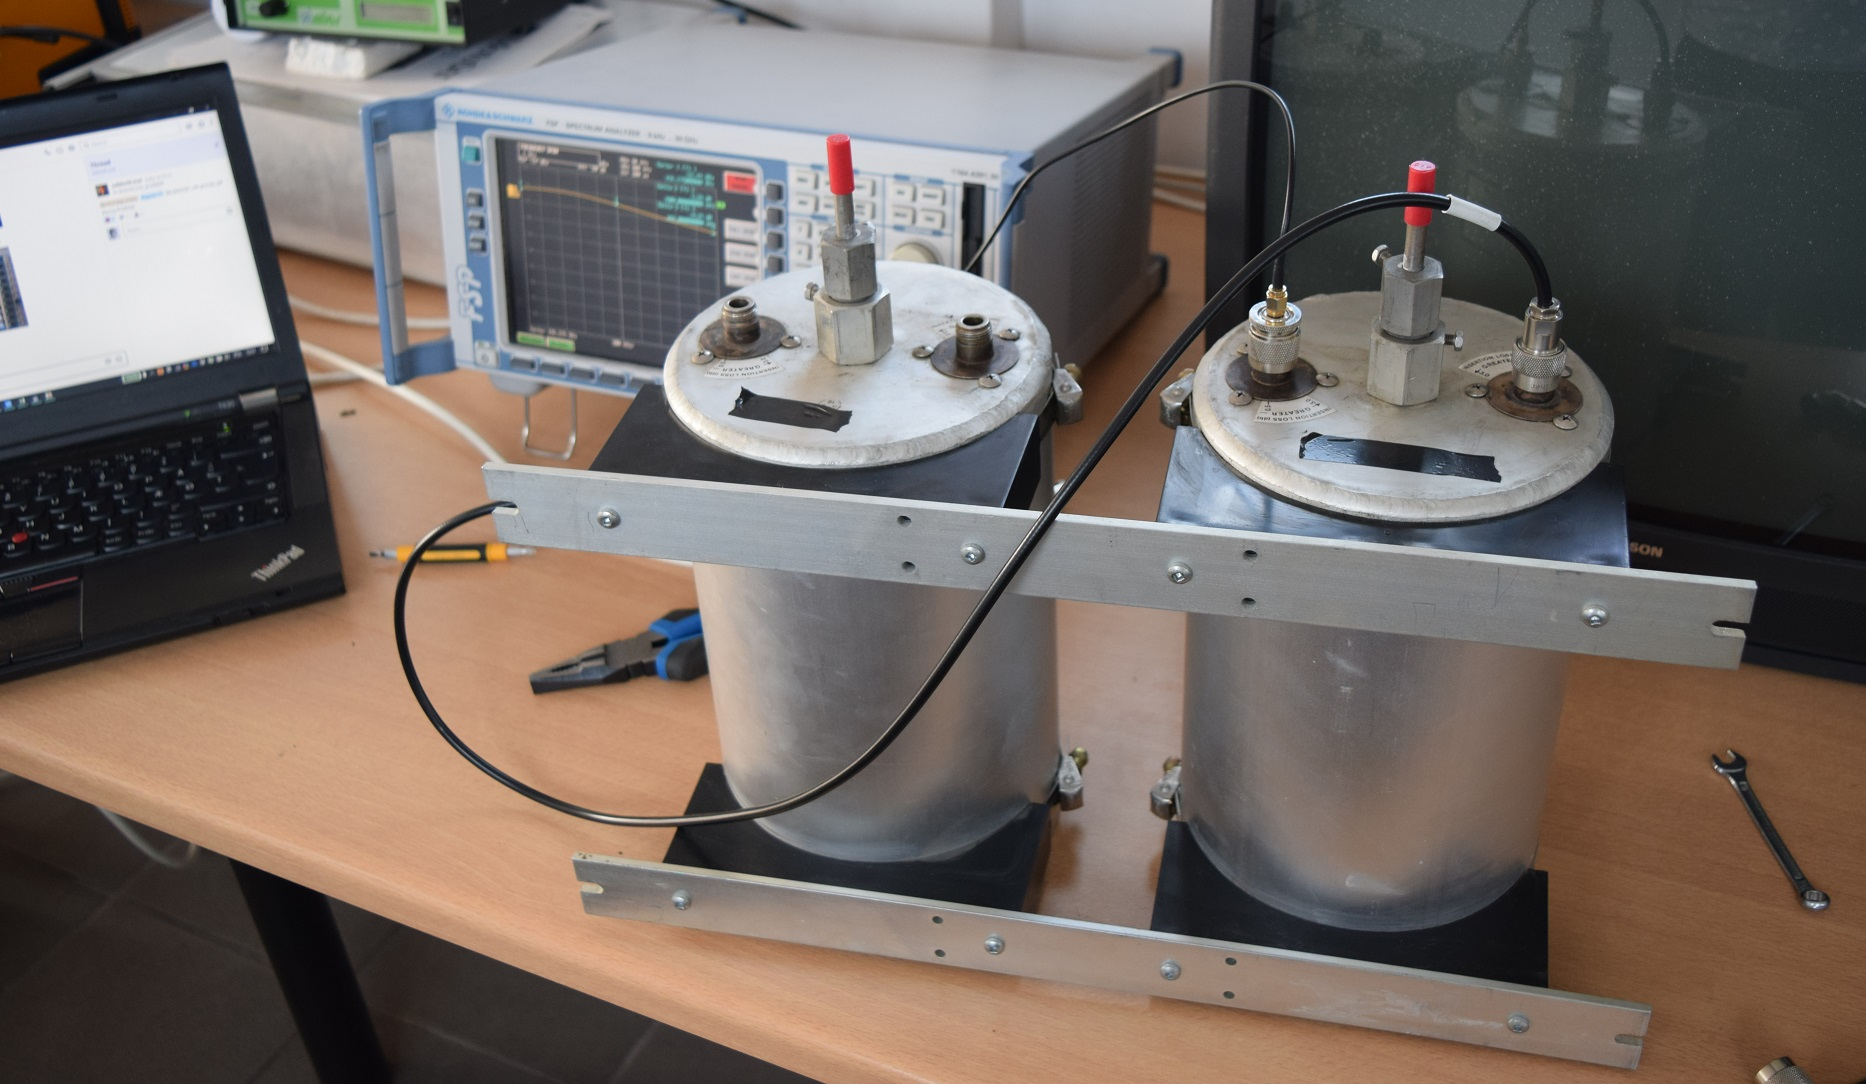
\includegraphics[width=0.5\paperwidth]{img/5/cavity_filter_during_tuning.jpg}
    \caption{Cavity filter during tuning}
    \label{cavity_filter_during_tuning}
\end{figure}

\begin{figure}
    \centering
    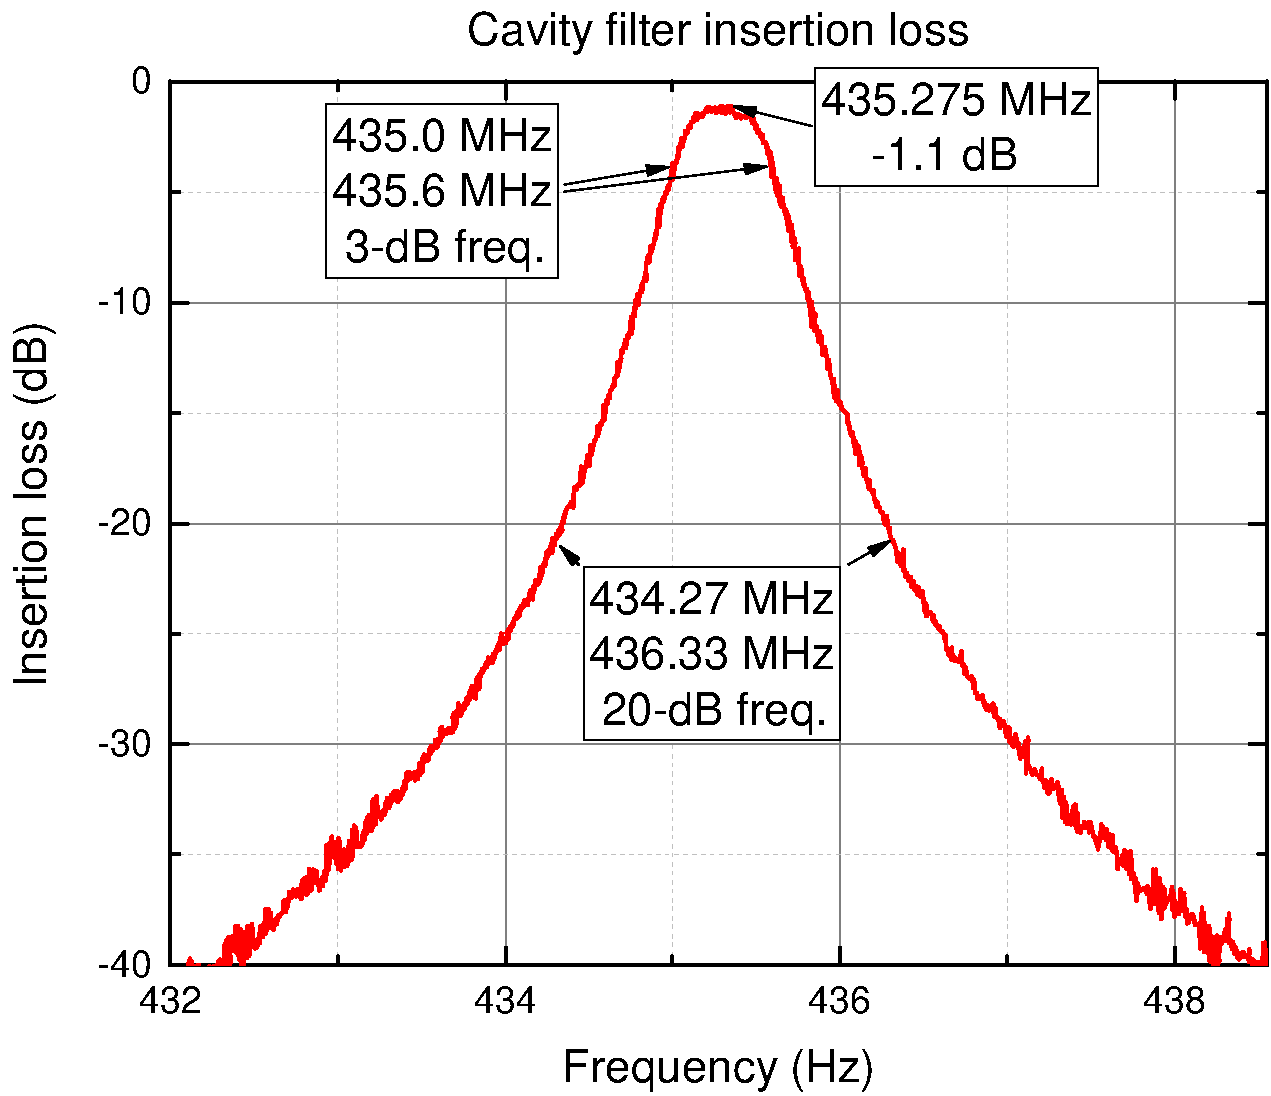
\includegraphics[width=0.5\paperwidth]{img/5/FilterLossG.pdf}
    \caption{Cavity filter insertion loss}
    \label{cavity_filter_insertion_loss}
\end{figure}

\begin{figure}
    \centering
    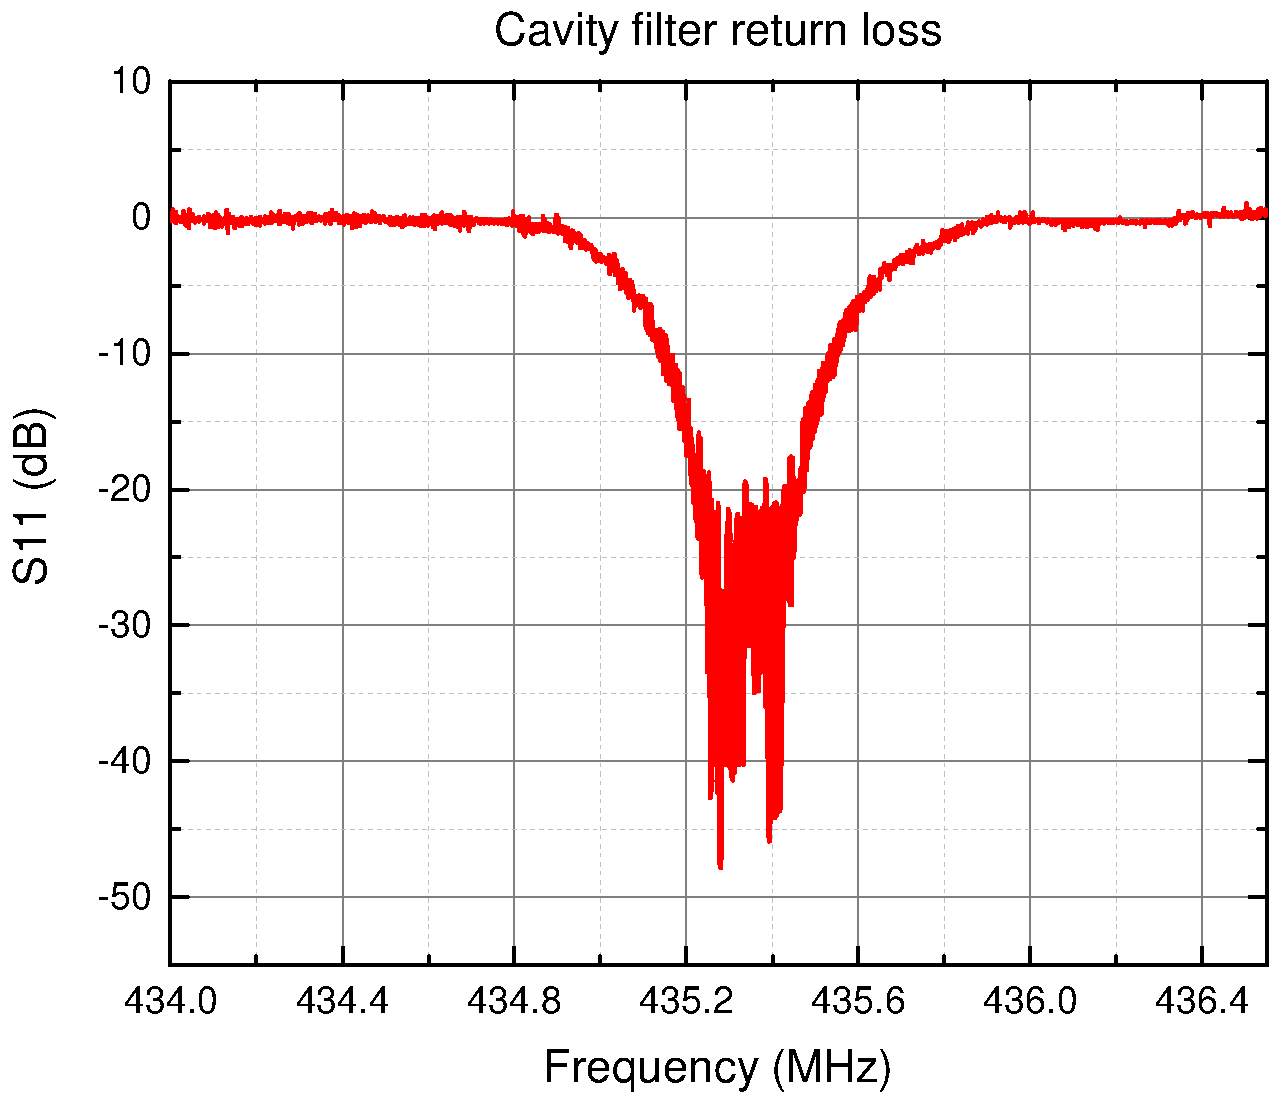
\includegraphics[width=0.5\paperwidth]{img/5/FilterMatchG.pdf}
    \caption{Cavity filter return loss}
    \label{cavity_filter_return_loss}
\end{figure}



\subsection{Low noise amplifier}
Low Noise Amplifier, installed close to the antenna reduces influence of the long cable attenuation between the antenna and the receiver and is designed to have low noise figure. According to the Friis formula, the total noise figure of the system will mostly depend on the insertion loss between the antenna and the noise figure of the Low Noise Amplifier. 

A dedicated Low Noise Amplifier was designed. As the main active component, a high-level Low Noise Amplifier: Mini-Circuits PGA-103+ \cite{lna_pga_datasheet} was used. Additional \SI{433}{\MHz} SAW filter was placed after the amplifier to reduce out of band harmonics and other unwanted products. Bias of the amplifier is created by RF Low Dropout Regulator Texas Instruments TPS7A47 \cite{lna_ldo_datasheet}. Amplifier was designed to support two-stage configuration, but for PW-Sat2 only first stage was populated. Schematic, PCB layout and the picture of the designed board are shown in the figures: \ref{lna_schematic} and \ref{lna_pcb}. The design is open source and all the source files can be found at \cite{lna_github}.

S-parameters of the LNA were tested using Rohde\& Schwarz ZVL Vector Network Analyser. Results are shown in the figure \ref{lna_s_params}. Achieved single-stage gain: \SI{17.5}{\dB} with \SI{8}{\MHz} bandwidth.

\begin{landscape}
\begin{figure}
    \centering
    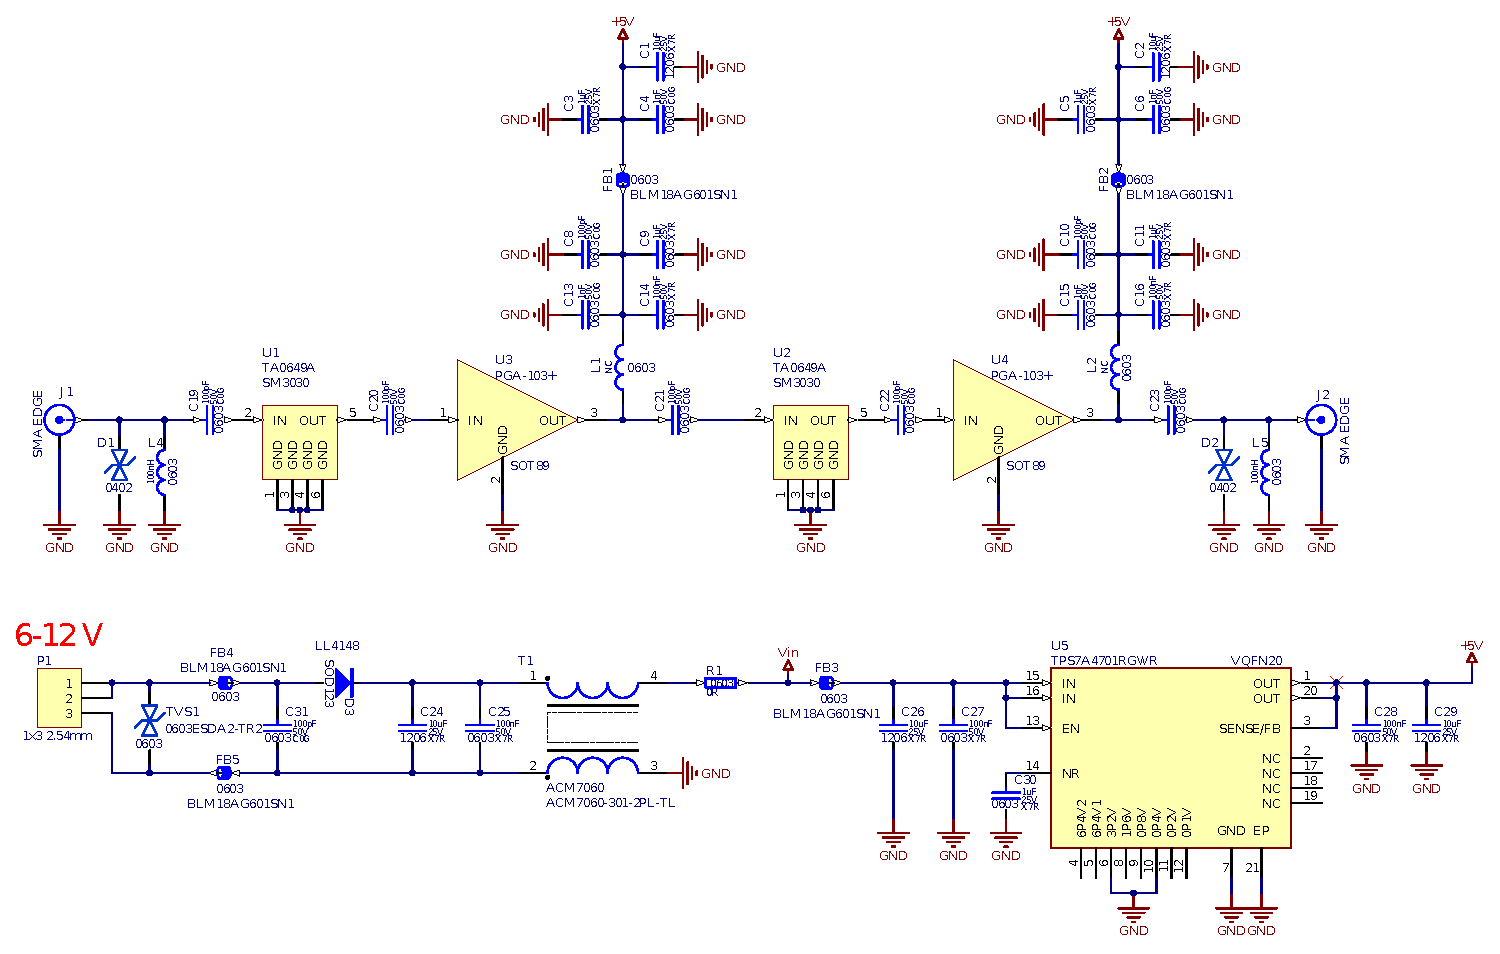
\includegraphics[width=1.12\paperwidth]{img/5/lna_schematic.eps}
    \caption{Low Noise Amplifier Schematic}
    \label{lna_schematic}
\end{figure}
\end{landscape}

\begin{figure*}
   \centering
\begin{tabular}{cc}
        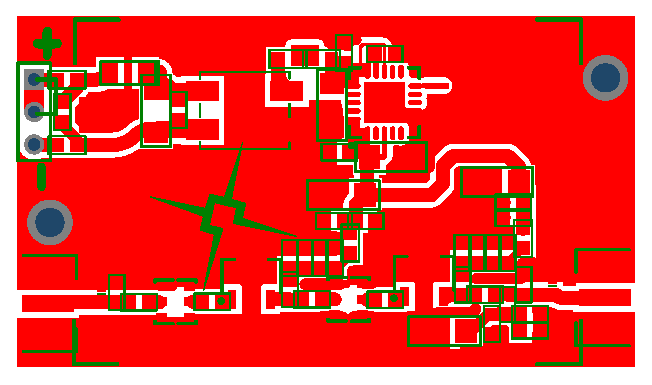
\includegraphics[width=0.4\paperwidth]{img/5/lna_pcb.eps}
    & 
        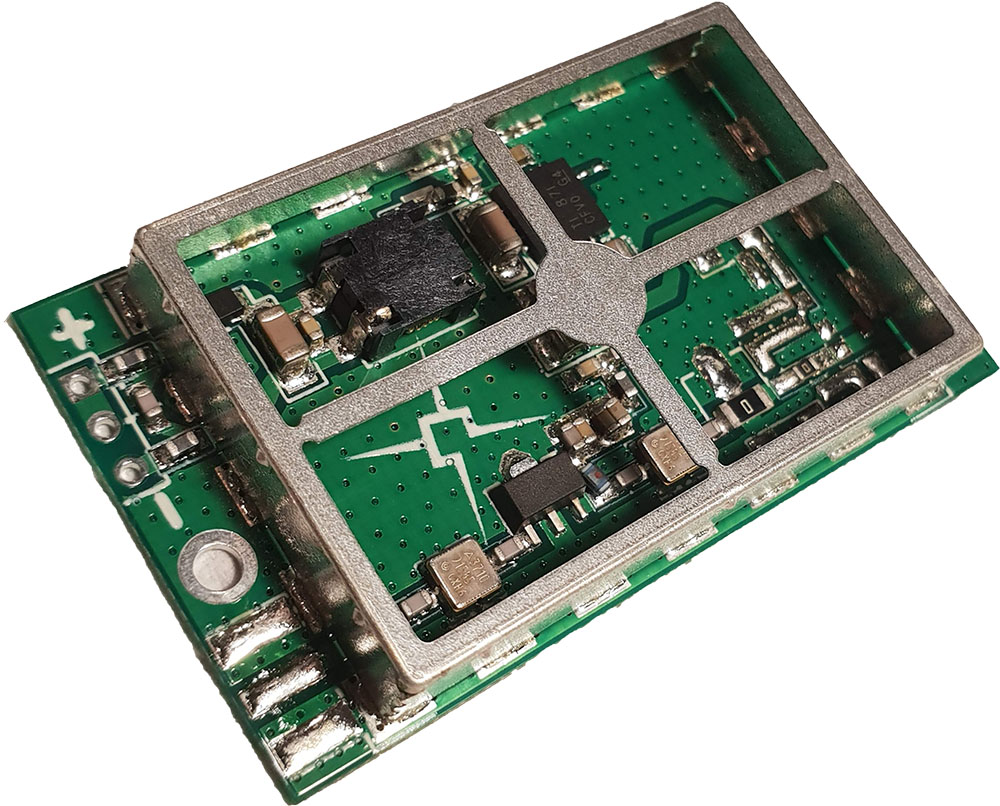
\includegraphics[width=0.3\paperwidth]{img/5/lna_assembled.jpg}
\end{tabular}
\label{lna_pcb}
\caption{Low Noise Amplifier PCB layout and assembled picture}
\end{figure*}

\begin{figure*}
   \centering
\begin{tabular}{cc}
        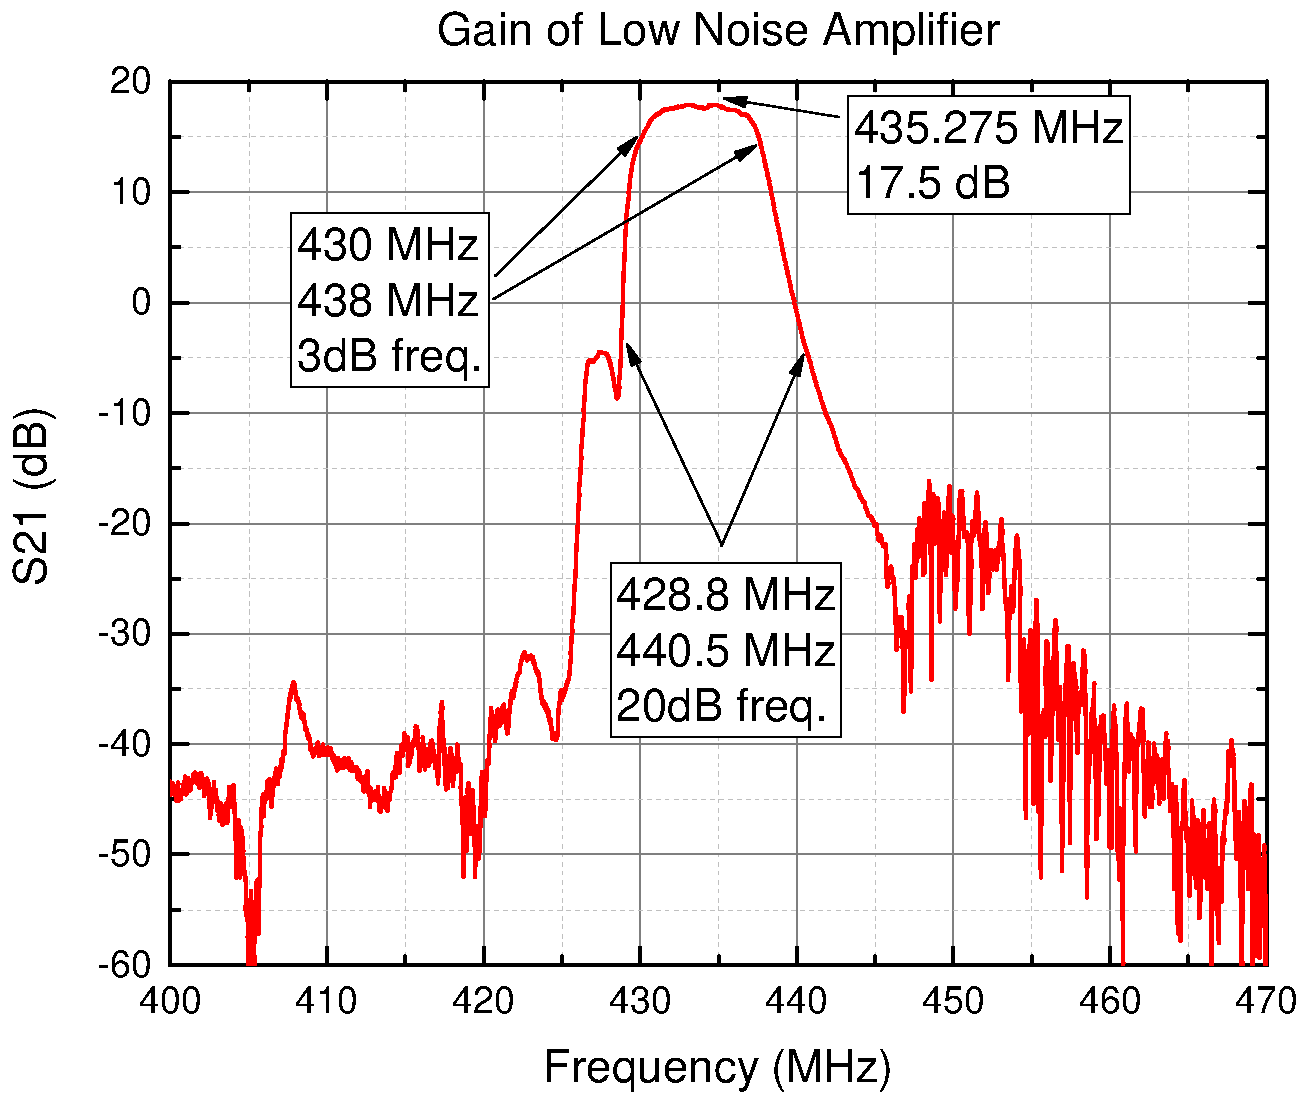
\includegraphics[width=0.35\paperwidth]{img/5/LnaGain.pdf}
    & 
        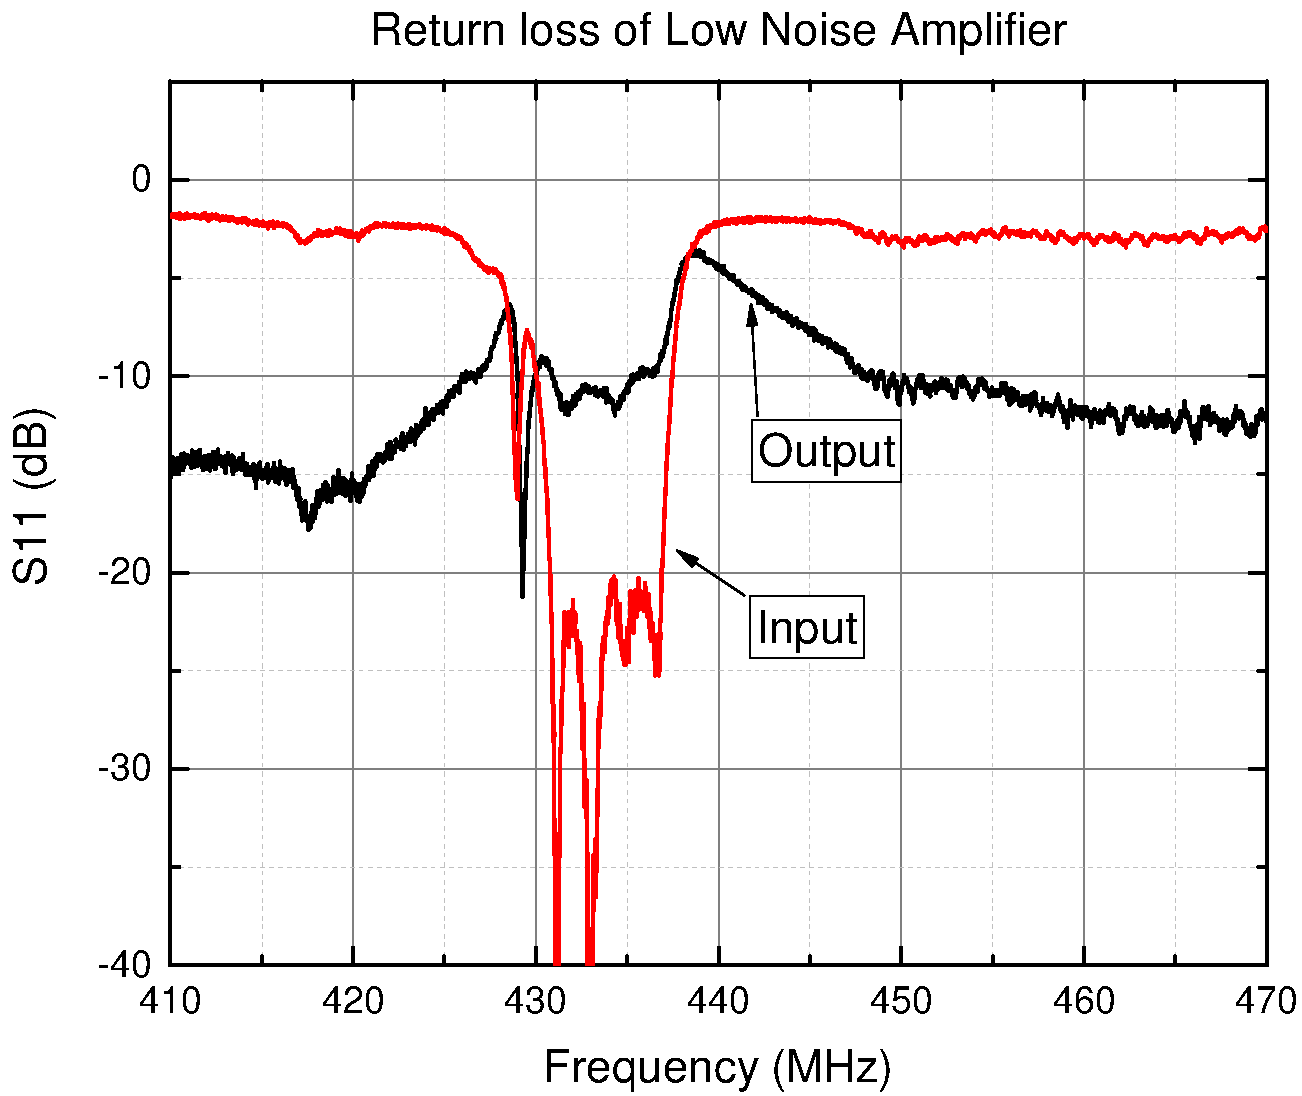
\includegraphics[width=0.35\paperwidth]{img/5/LnaMatch.pdf}
\end{tabular}
\label{lna_s_params}
\caption{Low Noise Amplifier S-parameters}
\end{figure*}


\subsection{Receiver}
Due to the custom packet format no commercially available integrated circuits were able to correctly receive packets, therefore a custom solution was required for de-modulation and packet recovery.
To receive BPSK signals, the phase recovery is necessary. One of the methods of the synchronous detection is the use of Costas loop \cite{costas_loop}. Most simple solution is to implement full signal chain: Costas loop, bit recovery and packet formatting using Digital Signal Processing on the baseband.

One of the possible and widely used methods is to use radio amateur transceiver in SSB mode - then radio acts as a multi-stage down-converter, allowing to receive baseband with audio card from PC. However, due to main purpose of transmitting audio signals, there is a lowpass filter for baseband at about \SI{3}{\kHz}. Using SSB mode for receiving PW-Sat2 is possible, however only for \SI{1.2}{\kbps} bitrate.

Another method was to use Software-Defined Radio, performing IQ downconversion and data transmission. The Radio Amateur Satellite Corporation designed an SDR receiver for their mission FUNcube Satellite. After mission success, they released their design and started selling FUNcube dongle shown in the figure \ref{funcube_pic}. Given that is was designed specifically for satellite communication and it was tested using similar CubeSat design, it was selected as the main receiver for PW-Sat2.

\begin{figure}
    \centering
    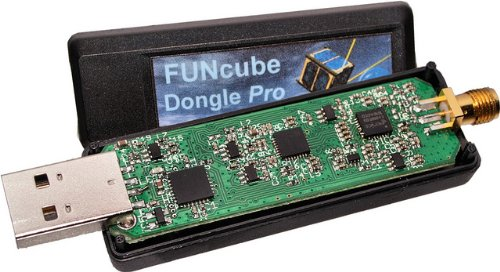
\includegraphics[width=0.6\paperwidth]{img/2/funcube.jpg}
    \caption{FUNcube Dongle Pro+. Source: \cite{funcube}}
    \label{funcube_pic}
\end{figure}

The receiver  functionalities:
\begin{itemize}
    \item Doppler correction,
    \item IQ data recording,
    \item BPSK demodulation,
    \item bit recovery,
    \item packet formatting,
    \item multiple bitrate simultaneous decoders,
    \item sending data on-line to the operators,
    \item work with different Software-Defined Radios and SSB transceivers
\end{itemize}

The block diagram of the designed system is shown in the figure \ref{demodulator_block_diagram}. All of the signal processing blocks were created using GNUradio framework.

\begin{figure}
    \centering
    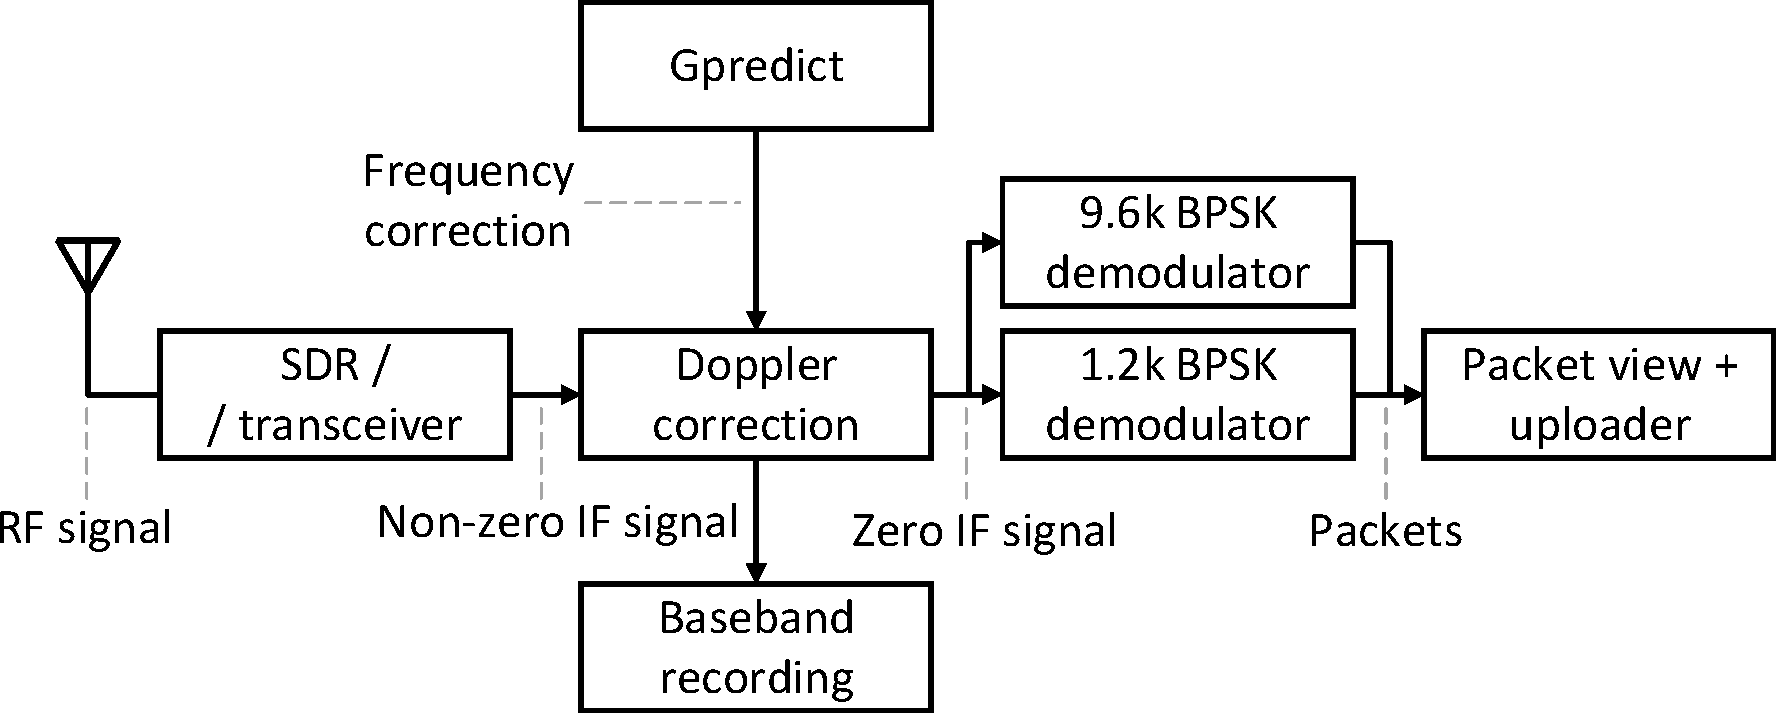
\includegraphics[width=0.6\paperwidth]{img/5/demodulator_block_diagram.pdf}
    \caption{Demodulator Block Diagram}
    \label{demodulator_block_diagram}
\end{figure}

First stage, the SDR / transceiver can be any type of Software-Defined radio working with osmocom device drivers, FUNcube SDR or analog SSB radio using audio card. To mitigate the DC-offset and IQ imbalance, the output of this block is on non-zero IF - the frequency of the PW-Sat2 is shifted from the LO frequency. For SSB transceiver, it has to be tuned \SI{2}{\kHz} below the center frequency due to the limited bandwidth of the audio filters, and for the SDR transceiver to eliminate the DC peak effect, the signal is shifted by 1/4 of the bandwidth. Signal source dialog of the main application is shown in the figure \ref{gs_source_selection}.

\begin{figure}
    \centering
    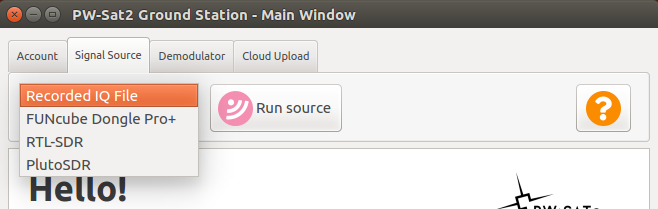
\includegraphics[width=0.6\paperwidth]{img/5/gs_source_selection.png}
    \caption{Ground station application - signal source selection}
    \label{gs_source_selection}
\end{figure}

Doppler correction is build on quadrature mixer and create zero-IF signal for the next processing blocks. Gpredict calculates required frequency shift and sends it to the block via TCP/IP connection. This updates local VCO frequency for the down-conversion. Latter, the signal is fist-stage filtered and saved to the file for logging purposes. GNUradio block diagram is shown in the figure \ref{gs_doppler_gnuradio}.

\begin{figure}
    \centering
    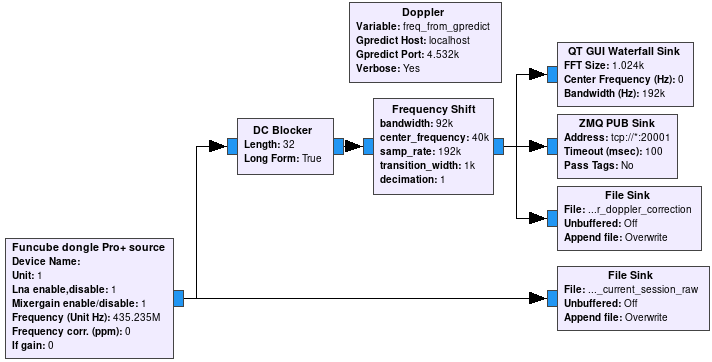
\includegraphics[width=0.7\paperwidth]{img/5/gs_doppler_gnuradio.png}
    \caption{Doppler correction block GNUradio flowgraph}
    \label{gs_doppler_gnuradio}
\end{figure}

In the system, there are two demodulators (for \SI{1.2}{\kbps} and \SI{9.6}{\kbps} bitrates) operating simulateneously. This allows immediate signal reception during bitrate change by the operator without any manual intervention in the software. This was achieved using GNURadio "hierarchial blocks". Top demodulator block is shown in the figure \ref{gs_demodulator_hier}, and each of Downlink blocks (Fig. \ref{gs_demodulator_diagram}) is a complete demodulator. The demodulator has its own GUI to show user the status of the block (carrier lock, bit lock, constellation diagram), shown the figure \ref{gs_demodulator_gui}.
Downlink receiver does the following operations:
\begin{itemize}
    \item resampling - to create a demodulator with selectable bitrate each of the bitrate decimates the input signal accordingly,
    \item Automatic Gain Control - the power of the signal should be constant as the tuning constants are dependent on the signal amplitude,
    \item Costas loop - carrier recovery and phase demodulation,
    \item filtering - low-pass signal with matched Root Raised Cosine filter to eliminate out of band noise and minimize Inter Symbol Interference,
    \item Symbol synchronization - recovers bits from the baseband signal,
    \item packet framing - builds a frame from stream of bits,
    \item frame pass to the higher level software.
\end{itemize}

\begin{figure}
    \centering
    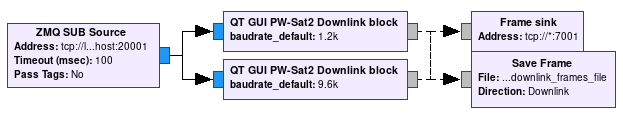
\includegraphics[width=0.7\paperwidth]{img/5/gs_downlink_hier.png}
    \caption{Hierarchial receiver GNUradio flowgraph}
    \label{gs_demodulator_hier}
\end{figure}

\begin{figure}
    \centering
    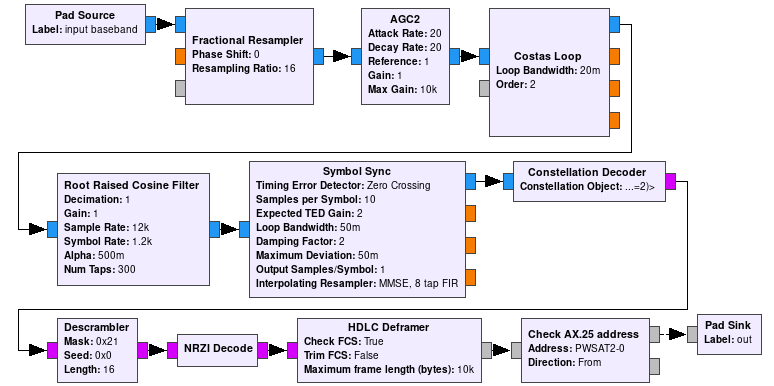
\includegraphics[width=0.7\paperwidth]{img/5/gs_demodulator_diagram.png}
    \caption{Ground station demodulator GNUradio flowgraph}
    \label{gs_demodulator_diagram}
\end{figure}

\begin{figure}
    \centering
    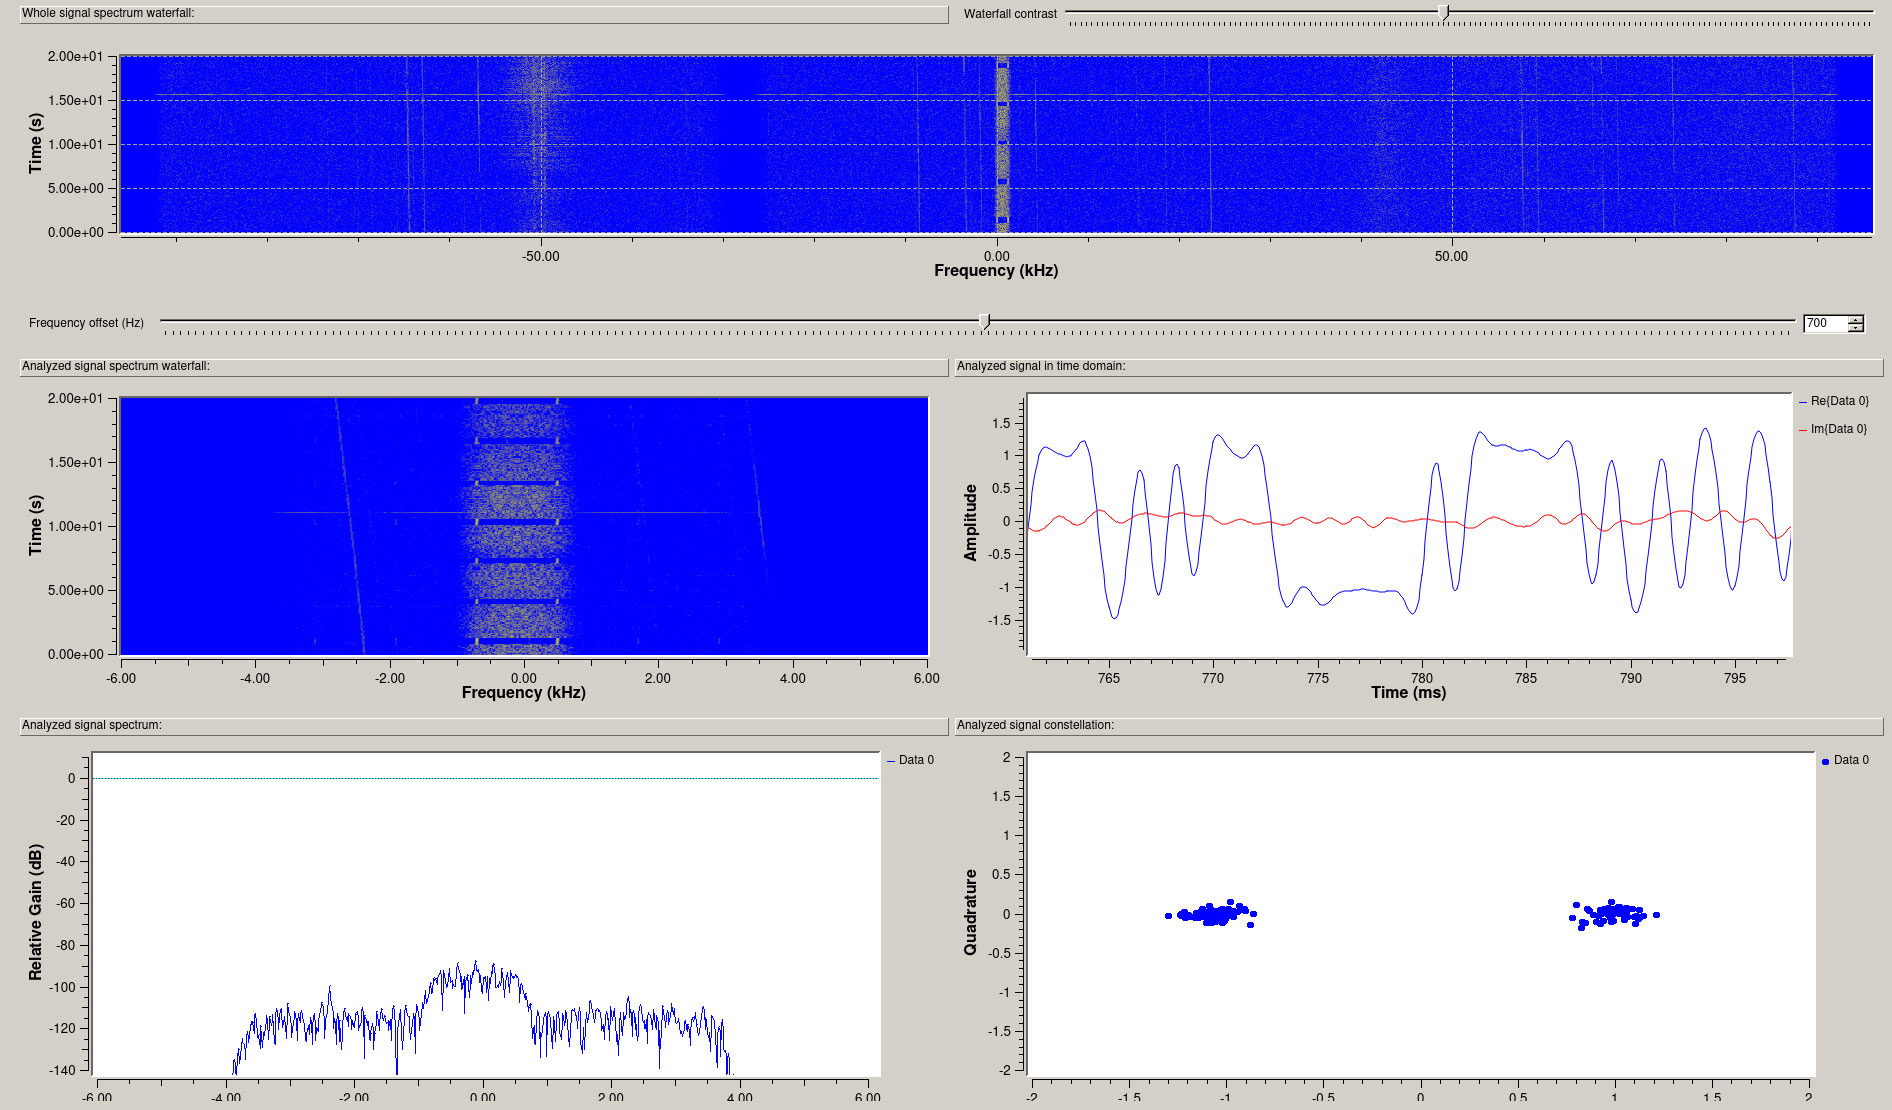
\includegraphics[width=0.7\paperwidth]{img/5/gs_demodulator_gui.jpg}
    \caption{Ground station demodulator GUI}
    \label{gs_demodulator_gui}
\end{figure}

The demodulator was designed for two major cases:
\begin{itemize}
    \item wide bandwidth and large frequency correction (when orbit Keppler data is not well-known, resulting in unpredicted Doppler shift),
    \item wide bandwidth and no frequency correction (when orbit Keppler data is well-known resulting in negligible frequency inaccuracies).
\end{itemize}

Depending on the case, different parameters of the Costas loop were determined. Both test-cases were implemented and the sensitivity and maximum frequency shift were determined.

After the packet reception, it is shown for the user (as in the figure \ref{gs_frame_view}) and uploaded to the cloud for further analysis by the operations team.

\begin{figure}
    \centering
    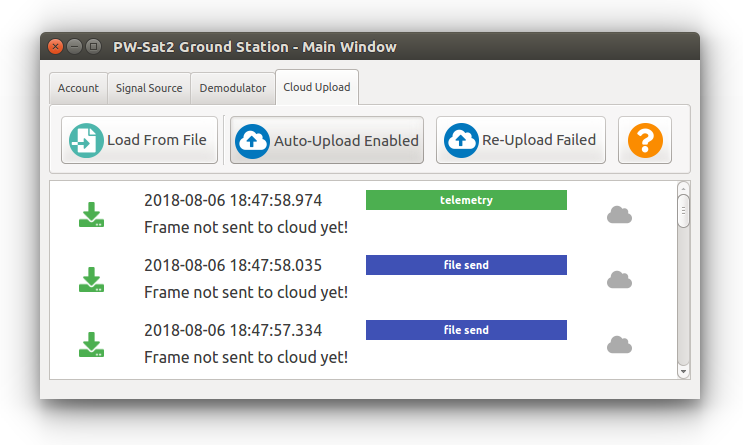
\includegraphics[width=0.6\paperwidth]{img/5/gs_frame_view.png}
    \caption{Ground station received frame view}
    \label{gs_frame_view}
\end{figure}


\subsubsection{Measurements}
Frequency correction block was tested using already flying satellites, verifying stability of frequency after correction.

The test setup for measuring demodulator is shown in the figure \ref{TODO}, and consist of:
\begin{itemize}
    \item PlutoSDR - transmitter of the frames with regulated center frequency and output power,
    \item attenuators
    \item Funcube Pro+ SDR - receiver used in the ground station
\end{itemize}

Frames to be transmitted were recorded with Software-Defined Radio during flatsat campaign and replayed during sensitivity tests. This ensures that all the important inadequacies transmitted by the radio transmitter were also taken into account.
With the test setup, sensitivity was automatically measured by varying output power of the transmitter (in \SI{0.25}{\dB} steps) and PER was recorded for each point. During the process, different parameters of the demodulator were tuned to increase the sensitivity. Final results are shown in the table \ref{TODO} and figures \ref{TODO} - \ref{TODO}.
